\documentclass[french]{book}
\usepackage[utf8x]{inputenc}
\usepackage[T1]{fontenc}
\usepackage{babel}
\usepackage{lmodern}
\usepackage[top=2cm,bottom=2cm,left=3cm,right=3cm]{geometry}
\usepackage{microtype}
\usepackage{mathtools, amssymb, amsthm}
\usepackage{mdframed}
\usepackage{hyperref}
\usepackage{graphicx}
\usepackage{xcolor}
\usepackage{mathrsfs}
\usepackage{wrapfig}
\usepackage{stmaryrd}
\usepackage{framed}
\usepackage{marginnote}
\usepackage[Glenn]{fncychap}
\usepackage[all]{xy}


\newtheorem{prototheorem}{Théorème}[section]
\newenvironment{thm}
   {\colorlet{shadecolor}{orange!10}\begin{shaded}\begin{prototheorem}}
   {\end{prototheorem}\end{shaded}}

\newtheorem{protocorollary}{Corollaire}
\newenvironment{corollary}
    {\colorlet{shadecolor}{violet!10}\begin{shaded}\begin{protocorollary}}
    {\end{protocorollary}\end{shaded}}

\newtheorem*{protolemma}{Lemme}
\newenvironment{lemma}
    {\colorlet{shadecolor}{pink!15}\begin{shaded}\begin{protolemma}}
    {\end{protolemma}\end{shaded}}

\theoremstyle{definition}
\newtheorem{protodefinition}{Définition}[section]
\newenvironment{definition}
    {\colorlet{shadecolor}{green!5}\begin{shaded}\begin{protodefinition}}
    {\end{protodefinition}\end{shaded}}

\newtheorem{protoproposition}{Proposition}[section]
\newenvironment{prop}
    {\colorlet{shadecolor}{blue!5}\begin{shaded}\begin{protoproposition}}
    {\end{protoproposition}\end{shaded}}

\theoremstyle{remark}
\newtheorem*{remark}{Remarque}
\newtheorem{exo}{Exercice}
\newtheorem*{protoexemple}{Exemple}
\newenvironment{exemple}
    {\colorlet{shadecolor}{gray!10}\begin{shaded}\begin{protoexemple}}
    {\end{protoexemple}\end{shaded}}


\newcommand{\lesss}{<}
\newcommand{\less}{\lesss}

\newcommand{\biggg}{>}
\newcommand{\bg}{\biggg}



\title{\bsc{Théorie des représentations}}
\date{2023-2024}
\author{Yves \bsc{Aubry}, M-147A, yves.aubry@univ-tln.fr, Joachim \bsc{Asch}}

\begin{document}

\maketitle

\tableofcontents

\part{Représentations linéaires des groupes finis}

\chapter{Généralités sur les groupes}

\section{Rappels}


Soit $G$ un groupe. Soit $H$ un sous-groupe de $G$ (i. e. $H \neq 0$ et $\forall x, y \in H, x y ^{-1} \in H$).

Considérons la relation binaire suivante sur $G$ :

Pour $x, y \in G$, $x \equiv _{d} y \mod H$ ssi $x y ^{-1} \in H$. C'est une relation d'équivalence. Elle est dite de congruence à gauche modulo $H$.

\begin{proof}
  En effet, si $x \in G$, alors $x x ^{-1} = e \in H$, donc $x \mod _{g} = x \mod H$. La relation est donc réflexive.

  De plus, si $x, y \in G$ tels que $x \equiv _{g} y \mod H$, alors $x y ^{-1} \in H$. $H$ étant un sous-groupe de $G$, il est donc stable par passage au symétrique. D'où $(x y ^{-1} ) ^{-1}  \in H$, i. e. $y x ^{-1} \in H$, c'est-à-dire $y \equiv _{g} x \mod H$.

  Enfin, si $x, y,z \in G$ tels que $x \equiv _{g} y \mod H$ et $y \equiv _{g} z \mod H$, alors $x y ^{-1} \in H$ et $yz ^{-1} \in H$. Or, $H$ étant un sous-groupe de $G$, donc $H$ est stable pour la loi de composition interne. D'où $(x y ^{-1} )(y z ^{-1} ) \in H$. Par associativité, $x (y y ^{-1} ) z ^{-1}  \in H$, ie $x z ^{-1}  \in H$.

  Donc $x \equiv _{g} z \mod H $ et la relation est transitive.
\end{proof}

\

Soit $x \in G$. La classe d'équivalence de $x$ pour cette relation d'équivalence est

\begin{gather*}
  cl _{d}(x) = \{ y \in G \mid x y ^{-1} \in H \} \\
  = \{ y \in G \mid \exists h \in H, x y ^{-1} = h \} \\
  = \{ y \in G \mid \exists h \in H, y = hx \} \\
  = \{ hx, h \in H \} =: Hx
\end{gather*}

De même, on considère, sur $G$,  la relation de congruence à gauche modulo $H$  :

\begin{equation*}
  x \equiv _{g} y \mod H \text{ ssi } x ^{-1} y \in H.
\end{equation*}

On montre de même que c'est une relation d'équivalence. Si $x \in G$, alors $cl_g(x) := xH = \{ xh, h \in H \} $.

\begin{remark}
  Si $G$ est abélien, alors les classes à gauche et à droite modulo $H$ co\"incident.
\end{remark}

\begin{definition}
  Un sous-groupe $H$ d'un groupe $G$ est dit distingué dans $G$ (ou normal) si :

  \begin{gather*}
    \forall  x \in G, xH = Hx, \\
    \text{ i. e. } \forall x \in G, x H x ^{-1}  \subset H \\
    \text{ i. e. } \forall x \in G, x H x ^{-1} =H.
  \end{gather*}
\end{definition}

On note alors $H \triangleleft G$.

\begin{remark}
  Tout sous-groupe d'un groupe abélien est distingué.
\end{remark}

\begin{prop}
  Soit $G$ un groupe et $H$ un sous-groupe distingué de $G$.

  On note $G/H$ l'ensemble des classes à droite ou à gauche modulo $H$.

  Si $x, y \in G$ et si l'on note $\overline{a} $ la classe de $a$ modulo $H$, on peut munir le quotient $G/H$ d'une structure de groupe en posant

  \begin{gather*}
    \overline{x} \cdot \overline{y} = \overline{xy}.
  \end{gather*}
\end{prop}

\begin{proof}
  Cette loi est bien définie, i. e. elle ne dépend pas du choix des représentants des classes d'équivalence.
\end{proof}

\begin{remark}
  Cette loi de la surjection canonique $\pi:
    \begin{array}{lll}
    G & \longrightarrow & G/H \\
    x & \longmapsto \overline{x}
    \end{array}$ un morphisme de groupes.
\end{remark}

\begin{thm}[Lagrange]
  Soit $G$ un groupe fini et $H$ un sous-groupe de $G$.

  Alors l'ordre de $H$ divise l'ordre de $G$.
\end{thm}

\begin{remark}
  L'ordre d'un groupe est simplement son cardinal.
\end{remark}

\begin{remark}
  Si $g$ est un élément de $G$, alors l'ordre de $G$ est défini comme l'ordre du sous-groupe $\langle g \rangle $ engendré par $g$. S'il est fini, alors l'ordre de $g$ est le plus petit entier $n$ tel que $g ^{n} =e$.

  D'après le théorème de Lagrange, l'ordre d'un élément divise l'ordre du groupe.
\end{remark}

\begin{remark}
  Si $G$ est un groupe fini et $H$ un sous-groupe de $G$, alors les classes (à gauche) modulo $H$ ont toutes le même cardinal, à savoir celui de $H$. En effet, l'application, pour $x \in G : f_x:
    \begin{array}{lll}
    H & \longrightarrow & xH \\
    h & \longmapsto xh
    \end{array}$ est bijective.
\end{remark}

\section{Exemples de groupes}

\subsection{$ (\mathbb{Z}, +)$ }

Groupe abélien.

$n \mathbb{Z} = \{ nk, k \in \mathbb{Z} \} $ est un sous-groupe de $\mathbb{Z}$.

\begin{remark}
  Tout sous-groupe de $\mathbb{Z}$ est de la forme $n \mathbb{Z}$ pour un certain $n \mathbb{Z}$.
\end{remark}

\subsection{$\mathbb{Z}/{ n }\mathbb{Z}$}

C'est l'ensemble des classes d'équivalence pour la relation d'équivalence suivante :

\begin{gather*}
  x, y \in \mathbb{Z}, x \equiv y \mod n \mathbb{Z} \text{ ssi } x - y \in n\mathbb{Z}.
\end{gather*}

\begin{remark}
  $\overline{x} = \overline{y}  $ ssi $x R y$.
\end{remark}

On munit l'ensemble quotient $\mathbb{Z}/{ n }\mathbb{Z}$ d'une structure de groupe (et même d'anneau) en posant, pour $x, y \in \mathbb{Z}$ : $\overline{x}+ \overline{y} = \overline{x+y}   $ (et $\overline{x} \times \overline{y} = \overline{x \times y}   $).

\begin{remark}
  $\mathbb{Z}/{ 6 }\mathbb{Z}$ anneau non intègre, car $ \overline{2} \times \overline{3} = \overline{0}   $.
\end{remark}

\begin{remark}
  $\mathbb{Z}/{ n }\mathbb{Z}$ est un corps ssi $n$ est premier.
\end{remark}

\begin{prop}
  Tous les groupes $\mathbb{Z}/{ n }\mathbb{Z}$ sont cycliques. Les générateurs sont les $\overline{a} $ tels que $a$ et $n$ sont premiers entre eux, i. e. $(a,n) = 1$. De plus, tout groupe cyclique est isomorphe à $\mathbb{Z}/{ n }\mathbb{Z}$ avec $n = \lvert G \rvert$.

  Enfin, si $G$ est cyclique d'ordre $n$ alors pour tout diviseur $d$ de $n$, $G$ admet un sous-groupe d'ordre $d$, et celui-ci est unique, et celui-ci est cyclique.
\end{prop}

\begin{remark}
  $\mathbb{Z}/{ 2 }\mathbb{Z} \times \mathbb{Z}/{ 3 }\mathbb{Z} = \{ (\overline{a}, \tilde{a} ), \overline{a} \in \mathbb{Z}/{ 2 }\mathbb{Z}, \tilde{a} \in \mathbb{Z}/{ 3 }\mathbb{Z}  \} $.
\end{remark}

\begin{thm}[Théorème des restes chinois]
  Soient $n_1, \dots, n_r$ des entiers premiers entre eux deux à deux. Alors l'application

  \[
  \begin{array}{lll}
  \mathbb{Z}/{ \prod_{i=1}^{r} n_i  }\mathbb{Z} & \longrightarrow & \prod_{i=1}^{r } \mathbb{Z}/{ n_i }\mathbb{Z}  \\
  a + (\prod_{i=1}^{r} n_i ) \mathbb{Z} & \longmapsto (a+ n_1 \mathbb{Z}, \dots, a+ n_r \mathbb{Z})
  \end{array}
  \]

  est un isomorphisme d'anneaux et la réciproque est vraie.
\end{thm}

\marginnote{19-09-2023}

\section{Groupe diédral}

Soit $n \geq 3$ un entier. Le groupe diédral de degré $n$ est le groupe des isométries du plan laissant fixe le polygone régulier à $n$ côtés. On le note $D_n$ (ou $D _{2n}$).

$D_n$ est un groupe d'ordre $2n$ constitué de $n$ rotations et de $n$ symétries.

Considérons le polygone régulier dont les sommets sont, dans le plan complexe, les $n$ racines $n$-ièmes de l'unité :

\[
e^{\frac{2ik \pi}{n}}, k = 0, 1, \dots, n-1.
\]

\begin{figure}[h!]
  \centering
  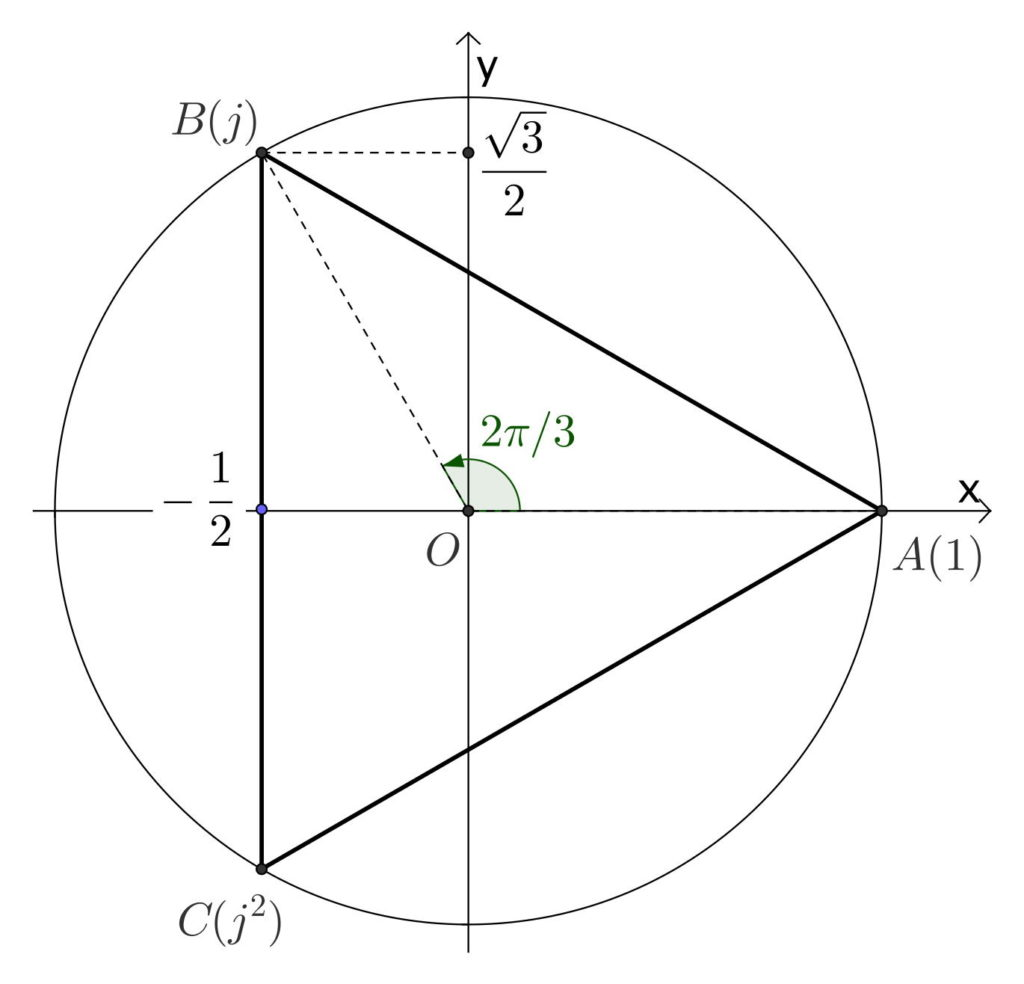
\includegraphics[scale=0.3]{figures/racines-3.jpg}
  \caption{Racines 3-ièmes de l'unité.}
  \label{}
\end{figure}

Soit $r = rot(0, \frac{2 \pi}{n})$ la rotation de centre $O$ et d'angle $\frac{2 \pi}{n}$ et soit $s$ la symétrie axiale d'axe la droite réelle $(x,x)$.

On a \[
r:\begin{array}{rcl}
\mathbb{C} & \longrightarrow & \mathbb{C} \\
z & \longmapsto e^{\frac{2 i \pi}{n}} z
\end{array}
\]

et

\[
s:
  \begin{array}{rcl}
  \mathbb{C} & \longrightarrow & \mathbb{C} \\
  z & \longmapsto \overline{z}
  \end{array}.
\]


On vérifie que l'on a $r ^{n} = 1 = id$, $s ^2 = 1 =id$ et $rs = r ^{-1} $.

\begin{proof}
  En effet, si $z \in \mathbb{C}$, alors

  \[
  r ^{-1} (z) = e^{- \frac{2 i \pi}{n}} z \text{ et } s r s(z) = s r (\overline{z} ) = s \left( e^{\frac{2 i \pi}{n}} \overline{z} \right) = e^{- \frac{2 i \pi}{n}} z = r ^{-1} (z),
  \]

  donc $s r s = r ^{-1} $.
\end{proof}

On peut donc définir le groupe diédral $D_n$ par ``générateurs et relations'' de la façon suivante :

\[
D_n = \langle r,s \rangle  \text{ avec } r ^{n} = s ^2 = 1 \text{ et } s r s = r ^{-1} .
\]

Le sous-groupe de $D_n$ engendré par $r$ est un sous-groupe d'ordre $n$ :

\[
\langle r \rangle = \{ r, r ^2, \dots, r ^{n-1}, id \} \simeq \mathbb{Z}/{ n }\mathbb{Z} .
\]

Il est d'indice 2 dans $D_n$, il est donc distingué dans $D_n$.

\subsection{Description du groupe $D_3$}

\begin{figure}[h!]
  \centering
  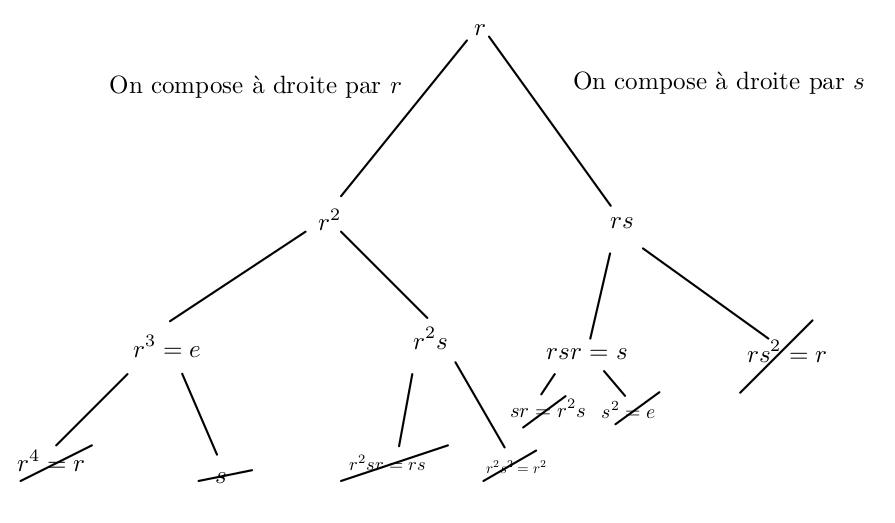
\includegraphics[scale=0.3]{figures/elts-d3.png}
  \caption{Description explicite des éléments de $D_3$.}
  \label{}
\end{figure}

On a donc

\[
D_3 = \{ e, r, r ^2, s, rs, r ^2 s \}
\]

\begin{remark}
  Il n'existe que deux groupes d'ordre 6 à isomorphisme près, à savoir le groupe cyclique (abélien) $\mathbb{Z}/{ 6 }\mathbb{Z}$ et le groupe symétrique (non abélien) $\mathfrak{S}_{3} $.
\end{remark}

Or $D_3$ n'est pas abélien, donc $D_3$ est isomorphe à $\mathfrak{S}_{3} $.

\begin{exo}
  Déterminer l'ordre des éléments de $D_3$ ainsi que ses sous-groupes.
\end{exo}

%\paragraph{Exemple du groupe quaternionien}

\begin{exemple}[Groupe quaternionien]
  Soit $\mathbb{H}$ le corps des quaternions d'Hamilton.

  \[
  \mathbb{H} = \{ a+ib+jc+kd \mid i ^2 = j ^2 = k ^2 = 1, ij = -ij = k, jk=-kj=i, ki=-ik=j \text{ et }  a, b, c, d \in \mathbb{R}\}.
  \]

  $\mathbb{H}$ est un corps non commutatif. On $\mathbb{R} \subset \mathbb{C} \subset \mathbb{H}$.

  Considérons le sous-ensemble suivant de $\mathbb{H}$ :

  \[
  \mathbb{H} _{8} = \{ 1, -1, i, -i, j, -j, k, -k \}.
  \]

  \begin{exo}
    Montrer que $\mathbb{H}_8$ muni de la multiplication est un groupe.
  \end{exo}

  C'est un groupe non abélien d'ordre 8.

  \begin{exo}
    Déterminer l'ordre des éléments de $\mathbb{H} _{8}$ ainsi que ses sous-groupes.
  \end{exo}
\end{exemple}



\paragraph{Rappel}


\begin{thm}[De classification des groupes abéliens finis]
  Tout groupe \textbf{abélien} fini est isomorphe à un produit de groupes cycliques de la forme

  \[
  \mathbb{Z}/{ d_1 }\mathbb{Z} \times \mathbb{Z}/{ d_2 }\mathbb{Z} \times \dots \times \mathbb{Z}/{ d_r }\mathbb{Z}, \text{ avec } d_1 \mid d_2 \mid \dots \mid d_r.
  \]

  Cette écriture est unique (à l'ordre près des facteurs).
\end{thm}

On en déduit qu'il existe trois groupes abéliens d'ordre 8 à isomorphisme près :

\[
\mathbb{Z}/{ 8 }\mathbb{Z}, \mathbb{Z}/{ 2 }\mathbb{Z} \times \mathbb{Z}/{ 4 }\mathbb{Z} \text{ et }  (\mathbb{Z}/{ 2 }\mathbb{Z}) ^3.
\]

Question : a-t-on $\mathbb{H}_8 \simeq D_4$ ?

\section{Les théorèmes de Sylow}

Si $H$ est un sous-groupe d'un groupe $G$, ses \textbf{conjugués} dans $G$ sont $g H g ^{-1} $, avec $g \in G$. En particulier, $H$ est distingué dans $G$ si et seulement si il est égal à tous ses conjugués.

\begin{definition}
  Si $G$ est un groupe fini d'ordre $p ^{\alpha} q$, avec $p$ premier, $\alpha \geq 1$ et $q$ premier avec $p$, alors tout sous-groupe de $G$ d'ordre $p3\alpha$ est appelé un $p$ sous-groupe de Sylow de $G$ (ou encore un $p$-Sylow de $G$).
\end{definition}

\begin{thm}[Premier théorème de Sylow]
  Soit $G$ un groupe d'ordre $p ^{\alpha} q$, $p$ premier, $\alpha \geq 1$, $(p, q)=1$. Pour tout $1 \leq \beta \leq \alpha$, il existe un sous-groupe de $G$ d'ordre $p ^{\beta}$.
\end{thm}

\begin{thm}[Deuxième théorème de Sylow]
  Le nombre $n_p$ de $p$-Sylow de $G$ vérifie :
  \[
  \begin{cases}
    n_p \equiv 1 \mod p \\
    n_p \mid q.
  \end{cases}
  \]
\end{thm}

\begin{thm}[Troisième théorème de Sylow]

  \

  \begin{enumerate}
    \item Le conjugué d'un $p$-Sylow est un $p$-Sylow.
    \item Tous les $p$-Sylow sont conjugués entre eux.
  \end{enumerate}
\end{thm}

\begin{exo}
  Montrer qu'il n'existe pas de groupes simples d'ordre 15.
\end{exo}

\begin{proof}
  Soit $G$ un groupe d'ordre $3 \times 5 = 15$. D'après le premier théorème de Sylow, $G$ admet au moins un 3-Sylow.

  Soit $n_3$ le nombre de 3-Sylow de G. Par le deuxième théorème de Sylow, on a

  \[
  n_3 \equiv 1 \mod 3 \text{ et } n_3 \mid 5.
  \]

  $G$ admet donc un unique 3-Sylow $H$.

  D'après le (1) du troisième théorème de Sylow, les conjugués de $H$ sont des 3-Sylow de $G$, donc sont égaux à $H$ puisque c'est le seul 3-Sylow de $G$. Donc $H$ est égal à tous ses conjugués et donc $H$ est distingué dans $G$. Puisque $\lvert H \rvert = 3$, $H \neq \{ e \} $ et $H \neq G$. Donc $G$ admet un sous-groupe distingué propre. Donc $G$ n'est pas simple.
\end{proof}

\subsection{Groupes agissant sur un ensemble ou action de groupes}

\begin{definition}[Action de groupe]
  Une action (à gauche) d'un groupe $G$ sur un ensemble $X$ est une application

  \[
  \begin{matrix}
  G  \times X& \longrightarrow & X \\
  (g,x) & \longmapsto & g \cdot x
  \end{matrix}
  \]

  telle que

  \begin{enumerate}
    \item $\forall x \in X, e \cdot x = x$ (où $e$ est l'élément neutre de $G$) ;
    \item $\forall g, g' \in G, \forall x \in X, g \cdot (g' \cdot x) = \underbrace{(gg')}_{\text{LCI de } G}\cdot x$.
  \end{enumerate}
\end{definition}

On peut voir une action comme un morphisme de groupes de $G$ dans le groupe symétrique $\mathfrak{S}_{X} $ de permutations dans $X$ :

\begin{prop}
  Si un groupe $G$ agit sur un ensemble $X$ par

  \[
    \begin{array}{rcl}
    G \times X & \longrightarrow & X \\
    (g,x) & \longmapsto g \cdot x,
    \end{array}
  \]

  alors pour tout $g \in G$, l'application

  \[
  \pi_g:
    \begin{array}{rcl}
    X & \longrightarrow & X \\
    x & \longmapsto g \cdot x
    \end{array}
  \]

  est une permutation de $X$ et l'application

  \[
  \pi:
    \begin{array}{rcl}
    G & \longrightarrow & \mathfrak{S}_{X}  \\
    g & \longmapsto \pi_g
    \end{array}
  \]

  est un morphisme de groupes.

  Réciproquement, si $
    \begin{array}{rcl}
    G & \longrightarrow & \mathfrak{S}_{X}  \\
    g & \longmapsto p_g
    \end{array}$ est un morphisme de groupes, alors $(g,x) \mapsto g \cdot x :=p_g(x)$ est une action de $G$ sur $X$.
\end{prop}

\begin{proof}

  \

  %Vérifions que $\pi$ est bien un morphisme de groupes. Montrons tout d'abord que, si $g \in G$, alors l'application

  %\[
  %\pi:
  %  \begin{array}{rcl}
  %  X & \longrightarrow & X \\
  %  x & \longmapsto \pi_g(x) = g \cdot x
  %  \end{array}
  %\]

  %est une permutation de $X$.

  %On a

  %\[
  %\pi_e:
  %  \begin{array}{rcl}
  %  X & \longrightarrow & X \\
  %  x & \longmapsto x
  %  \end{array} = id_X.
  %\]

  %De plus, si $g, g' \in G$, alors $\pi _{gg'} = \pi_g \circ \pi _{g'}$.

  %Soit $x \in X$, on a $\pi _{gg'}(x) = (gg') \cdot x$ et

  %\begin{gather*}
  %  (\pi_g \circ \pi _{g'})(x)= \pi_g(\pi _{g'})(x)
  %\end{gather*}

  Supposons que $G$ agisse sur un ensemble $X$ par $
    \begin{array}{rcl}
    G \times X & \longrightarrow & X \\
    (g,x) & \longmapsto g \cdot x
    \end{array}$.

  Soit $g \in G$. Considérons l'application $\pi_g:
    \begin{array}{rcl}
    X & \longrightarrow & X \\
    x & \longmapsto g \cdot x
    \end{array}$.

  Montrons que $\pi_g$ est injective. Soient $x, y \in X$ tq $\pi_g(x) = \pi_g(y)$. D'où $g \cdot x = g \cdot y$. D'où $g ^{-1}  \cdot g \cdot x = g ^{-1}  \cdot g \cdot y$. D'où $(g ^{-1}  g ) \cdot x = (g ^{-1}  g ) \cdot y$. D'où $e \cdot x = e \cdot y$. Donc $\pi_g$ est injective. Montrons que $\pi_g$ est surjective. Soit $y \in X$. On a $y = \pi_g(g ^{-1}  y) = g \cdot g ^{-1}  \cdot y$. Donc $\pi_g$ est surjective. Donc $\pi_g$ est bijective.

  On peut donc considérer l'application $\pi:
    \begin{array}{rcl}
    G & \longrightarrow & \mathfrak{S}_{X}  \\
    g & \longmapsto \pi_g
    \end{array}$.

  Montrons que $\pi$ est un morphisme de groupes. Montrons que $\forall g, g' \in G, \pi _{g g'} = \pi_g \circ \pi _{g'}$.

  Soient $g, g' \in G$. Soit $x \in X$. $$\pi _{ gg'}(x) = (g g') \cdot x = g \cdot g' \cdot x = g \cdot (\pi _{ g'} (x)) = \pi_g (\pi _{ g'}(x)).$$

  Donc $\pi _{ gg'} = \pi_g \circ \pi _{ g'}$.

  \

  Réciproquement, si on se donne un morphisme de groupes d'un groupe $G$ dans un groupe de permutations $\mathfrak{S}_{X} $ :

  \[
  p:
    \begin{array}{rcl}
    G & \longrightarrow & \mathfrak{S}_{X}  \\
    g & \longmapsto p_g,
    \end{array}
  \]

  alors l'application

  \[
    \begin{array}{rcl}
    G \times X & \longrightarrow & X \\
    (g,x) & \longmapsto g \cdot := p_g(x)
    \end{array}
  \]

  est une action de groupes.

  En effet,

  \begin{enumerate}
    \item Soit $x \in X$, on a $e \cdot x = p_e(x) = id_X(x) = x$, car $p$ est un morphisme de groupes et l'image de l'élément neutre par un morphisme de groupes est l'élément neutre.
    \item Soient $g, g' \in G$ et soit $x \in X$ ; on a

    \begin{gather*}
      g \cdot (g' \cdot x) = g \cdot (p _{g'}(x)) = p_g(p _{g'}(x)) = (p_g \circ p _{g'})(x) = p _{gg'}(x) = (gg') \cdot x,
    \end{gather*}

    car $p$ est un morphisme de groupes.
  \end{enumerate}
\end{proof}

Cela établit deux bijections réciproques entre l'ensemble des actions de $G$ sur $X$ et celui des morphismes de $G$ dans $\mathfrak{S}_{X} $.

\begin{definition}
  Si un groupe $G$ agit sur un ensemble $X$, alors la relation sur $X$ définie par : pour $x, y \in X, x \sim y $ ssi $\exists g \in G, y = g  \cdot x$ est une relation d'équivalence. La classe d'équivalence de $X$ pour cette relation s'appelle \textbf{l'orbite} de $X$ :

  \[
  Orb(x):= \{ g \cdot x, g \in G \} .
  \]

  Ainsi, l'ensemble des orbites forme une \textbf{partition} de $X$.

  On dit que $g$ agit \textbf{transitivement} s'il n'y a qu'une seule orbite.

  Le \textbf{noyau} de l'action est le noyau du morphisme associé :

  \[
  \pi:
    \begin{array}{rcl}
    G & \longrightarrow & \mathfrak{S}_{X}  \\
    g & \longmapsto \left(\pi_g:
      \begin{array}{rcl}
      X & \longrightarrow & X \\
      x & \longmapsto g \cdot x
      \end{array}\right)
    \end{array}
  \]

  \[
  \operatorname{Ker}(\pi) = \{ g \in G \mid \forall x \in X, g \cdot x = x \}.
  \]

  On dit que l'action est \textbf{fidèle} si son noyau est réduit à $\{ e \} $ (i. e. si le morphisme $\pi$ est injectif).

  Le \textbf{stabilisateur} (ou groupe d'isotropie) d'un élément $x \in X$ est l'ensemble :

  \[
  Stab(x) = \{ g \in G \mid g \cdot x = x \}.
  \]

  C'est un sous-groupe de $G$ (en exercice).
\end{definition}

\begin{prop}
  Pour $x$ fixé dans $X$, l'application

  \[
    \begin{array}{rcl}
    G & \longrightarrow & X \\
    g & \longmapsto g \cdot x
    \end{array}
  \]

  définit une bijection de l'ensemble $G / Stab(x)$ des classes à gauche modulo $Stab(x)$ sur l'orbite de $x$. Ainsi, le cardinal de l'orbite $Orb(x)$ est égal à l'indice du stabilisateur de $x$ :

  \[
  \sharp(Orb(x)) = [G:Stab(x)].
  \]
\end{prop}

\begin{thm}[Formule des classes]
  Soit $G$ un groupe fini agissant sur un ensemble fini $X$. Alors

  \[
  \sharp(X) = \sum_{\substack{x \text{ décrivant un système} \\ \text{des représentants des orbites} }}^{} [G:Stab(x)].
  \]
\end{thm}

\begin{proof}
  \[
  \sharp(X) = \sum_{i=1}^{m} \sharp(Orb(x_i)),
  \]

  où $\{ x_1, \dots, x_n \}$ est un système des représentants des orbites pour l'action de $G$ sur $X$.
\end{proof}

\paragraph{Exemple d'action de groupe}

 On fait agit un groupe $G$ sur lui-même par conjugaison

 \[
   \begin{array}{rcl}
   G \times G & \longrightarrow & G \\
   (g,x) & \longmapsto g \cdot x := g x g ^{-1} .
   \end{array}
 \]

C'est bien une action de groupes, car

\begin{enumerate}
  \item Soit $x \in G$, on a $e \cdot x = e x e ^{-1} =x$.
  \item Soient $g, g' \in G$ et $x \in G$. On a :

  \[
  g \cdot (g' \cdot x) = g \cdot (g x g ^{-1} )=g(g'x (g')^{-1} ) g ^{-1} = (gg') x ((g')^{-1} g ^{-1} ) = (gg')x(gg') ^{-1} = (gg')\cdot x.
  \]
\end{enumerate}

\emph{Cette action est-elle transitive, fidèle ? Quelle est l'orbite d'un élément ?}\marginnote{20-09-2023}


Soit $x \in G$. L'orbite de $x$ est :

\[
Orb(x) = \{ g \cdot x, g \in G \} = \{ g x g ^{-1} , g \in G \} = \text{classe de conjugaison de } x \text{ dans } G.
\]

On a $Orb(e) = \{ e \} $. Si $G$ n'est pas réduit à $\{ e \} $, il y a plusieurs orbites : l'action n'est donc pas transitive (il y a autant d'orbites que de classes de conjugaison).

\emph{L'action est-elle fidèle ?}  Etudions le noyau du morphisme $\pi$ associé à cette action

\[
\pi:
  \begin{array}{rcl}
  G & \longrightarrow & \mathfrak{S}_{G}  \\
  g & \longmapsto \left( \pi_g:
    \begin{array}{rcl}
    G & \longrightarrow & G \\
    x & \longmapsto g x g ^{-1}
    \end{array}\right).
  \end{array}
\]

On a

\begin{gather*}
  \operatorname{Ker}(\pi) = \{  g \in G \mid \pi_g =id_G \} = \{ g \in G \mid \forall x \in G, \pi_g(x) = x \} \\
  = \{ g \in G \mid \forall x \in G, g x g ^{-1} =x \} =  \{ g \in G \mid \forall x \in G, gx = xg \} = Z(G).
\end{gather*}

L'action est fidèle si et seulement si le centre de $G$ est réduit à l'élément neutre.

Soit $x \in G$. \emph{Quel est le stabilisateur de $x$ ?}

\begin{gather*}
  Stab(x) = \{ g \in G \mid g \cdot x = x \} = \{ g \in G \mid g x g ^{-1} =x \} = \{ g \in G \mid gx=xg \} = \text{centralisateur de } x.
\end{gather*}

Etudions un exemple avec $G = \mathfrak{S}_{3} $. Les orbites de $\mathfrak{S}_{3} $ pour cette action sont les classes de conjugaison de $\mathfrak{S}_{3} $. Elles constituent une partition de $\mathfrak{S}_{3} $.

\begin{enumerate}
  \item $Orb(e) = \{ e \} $.
  \item $Orb(\tau_3) = \{ \sigma \tau_3 \sigma ^{-1} , \sigma \in \mathfrak{S}_{3}  \} = \{ \text{transpositions de } \mathfrak{S}_{3} \} = \{ \tau_1, \tau_2, \tau_3 \} $.
  \item $Orb(\sigma_1) = \{ \sigma \sigma_1 \sigma ^{-1} , \sigma \in \mathfrak{S}_{3}  \} = \{ 3-\text{cycles de } \mathfrak{S}_{3}  \} = \{ \sigma_1, \sigma_2 \} $.
\end{enumerate}

La formule des classes s'écrit alors :

\[
\lvert \mathfrak{S}_{3} \rvert = \sum_{}^{} [\mathfrak{S}_{3}: Stab(x_i)],
\]

où $\{ x_1, x_2, x_3 \} $ est un système des représentants de l'orbite, avec $x_1 = e, x_2 = \tau_1, x_3 = \sigma_1$.

On a

\[
\lvert \mathfrak{S}_{3}  \rvert = \sum_{i=1}^{3} \sharp Orb(x_i)  =  \sharp Orb(x_1) +\sharp Orb(x_2) + \sharp Orb(x_3) =1+3+2 = 6.
\]

L'action est fidèle, car $Z(\mathfrak{S}_{3} ) = \{ e \} $. L'action n'est pas transitive, car il y a trois orbites, à savoir les trois classes de conjugaison.

\[
Stab(e) = \{ \sigma \in \mathfrak{S}_{3} \mid \sigma e = e \sigma \}= \mathfrak{S}_{3}.
\]

On a bien

\begin{gather*}
  [\mathfrak{S}_{3}: Stab(e) ] = \frac{\lvert \mathfrak{S}_{3}  \rvert}{\lvert Stab(e) \rvert} = \frac{3!}{3!}=1 = \sharp Orb(e).
\end{gather*}

On a $[\mathfrak{S}_{3}: Stab(\tau_3) ] = \sharp Orb(\tau_3) = 3$, donc $\lvert Stab(\tau_3) \rvert = 2$. D'où

\begin{gather*}
  Stab(\tau_3) = \{ \text{permutations de } \mathfrak{S}_{3} \text{ qui commutent avec } \tau_3 \} = \{ e, \tau_3 \}.
\end{gather*}

On a $[\mathfrak{S}_{3}: Stab(\sigma_1) ] = \sharp Orb(\sigma_1)=2$, donc $\lvert Stab(\sigma_1) \rvert = 3$. Puisque l'indice du stabilisateur est 2, on en déduit que $Stab(\sigma_1) \triangleleft \mathfrak{S}_{3} $. Or les seuls sous-groupes distingués de $\mathfrak{S}_{n} $ sont $\{ e \}, \mathfrak{S}_{n} \text{ et }  \mathfrak{A}_n  $. Donc

\begin{gather*}
  Stab(\sigma_1) = \mathfrak{A}_3 = \{ e, \sigma_1, \sigma_2 \}.
\end{gather*}

\chapter{Représentations linéaires des groupes finis}

Théorie introduite par Frobenius à la fin du XIX siècle.

\section{Premières définitions}

\begin{definition}
  Une représentation linéaire d'un groupe $G$ est la donnée d'un $\mathbb{C}$-espace vectoriel $V$ muni d'une action de groupes (à gauche) de $G$ agissant de manière linéaire :

  \[\begin{matrix}
    G \times V & \longrightarrow & V \\
    (g,x) & \longmapsto & g \cdot x
  \end{matrix}\]
  %  \begin{array}{rcl}
  %  G \times V & \longrightarrow & V \\
  %  (g,x) & \longmapsto g \cdot x
  %  \end{array}

  telle que

  \begin{enumerate}
    \item $\forall x \in V, e \cdot x = e$ ;
    \item $\forall g, g' \in G, \forall x \in V, g \cdot (g' \cdot x) = (gg')\cdot x$ ;
    \item $\forall g \in G, \forall x,x' \in V, \forall \lambda, \lambda' \in \mathbb{C}$, $g \cdot (\lambda x+\lambda'x') = \lambda g \cdot x + \lambda' g \cdot x$.
  \end{enumerate}
\end{definition}

Une représentation linéaire d'un groupe $G$ est donc la donnée d'un $\mathbb{C}$-espace vectoriel $V$ et d'un morphisme de groupes :

%\[
%\rho:
%  \begin{array}{rcl}
%  G & \longrightarrow & GL(V) \\
%  g & \longmapsto \left(\rho_g:
%    \begin{array}{rcl}
%    V & \longrightarrow & V \\
%    x & \longmapsto g \cdot x
%    \end{array}\right),
%  \end{array}
%\]


\[\begin{matrix}
\rho : & G & \longrightarrow & GL(V) \\
\ & g & \longmapsto & \left(\begin{matrix}
 V & \longrightarrow & V \\
 x & \longmapsto & g \cdot x
\end{matrix}\right)
\end{matrix}\]
où $GL(V)$ est le groupe des automorphismes du $\mathbb{C}$-espace vectoriel $V$.

On a bien $\forall g, g' \in G, \rho _{gg'} = \rho_g \circ \rho _{g'}$ et $\rho_e=id_V$ et $\rho _{g ^{-1} } = \rho_g ^{-1} $ comme vu précédemment.

De plus, $\forall  g \in G, $ la bijection $\rho_g$ est un endomorphisme de $V$, i. e. une application linéaire de $V$ dans $V$ et donc $\rho_g \in GL(V)$. En effet, si $x, x' \in V$ et $\lambda , \lambda' \in \mathbb{C}$, alors

\begin{gather*}
  \rho_g(\lambda x + \lambda' x') = g \cdot(\lambda x+ \lambda'x') \stackrel{(3)}{=} \lambda g \cdot x + \lambda' g \cdot x' = \lambda \rho_g(x) + \lambda'\rho_g(x').
\end{gather*}

\begin{definition}
  L'espace vectoriel $V$ est appelé \textbf{l'espace de la représentation}.

  La dimension de $V$ (en tant que $\mathbb{C}$-espace vectoriel) est appelé le \textbf{degré} ou la dimension de la représentation.

  Lorsque $\rho$ est injectif, la représentation est dite \textbf{fidèle} ; le groupe $G$ se représente alors de manière concrète comme un sous-groupe de $GL(V)$ ; lorsque $V$ est de dimension finie (ce que nous allons supposer dorénavant), le choix d'une base du $\mathbb{C}$-espace vectoriel $V$ fournit alors une représentation encore plus concrète comme groupe de matrice.
\end{definition}

\begin{remark}[Personnelle]
  Si \(\rho\) est une représentation fidèle, alors

  \[\operatorname{Ker}(\rho) = \{ g \in G \mid \forall x \in V, g \cdot x = x \} = \{ e \}. \]
\end{remark}

\begin{remark}
  Soient $G$ un groupe fini et $\rho : G \to GL(V)$ une représentation (linéaire) de $G$. Soit $g \in G$ un élément d'ordre $n$. On a alors

  \[
  (\rho_g)^n = \rho _{g ^{n}} = \rho_e = id_V.
  \]

  Donc l'endomorphisme $\rho_g$ est racine du polynôme $X^{n}-1$ qui n' a que des racines simples. Le polynôme minimal de $\rho_g$ divise donc le polynôme $X ^{n}-1$ et n'a donc aussi que des racines simples. Le polynôme minimal de $\rho_g$ est donc scindé sur $\mathbb{C}$ et à racines simples, on en déduit que l'endomorphisme de $\rho_g$ est \textbf{diagonalisable}.
\end{remark}

%\paragraph{Exemples de représentations}

\begin{exemple}[De représentations]

  \

  \begin{enumerate}
    \item La représentation triviale (ou représentation unité) :

    \[\begin{matrix}
    \rho : & G & \longrightarrow & GL(\mathbb{C}) \simeq \mathbb{C}^{*} \\
    \ & g & \longmapsto & \left( \rho_g : \begin{matrix}
     \mathbb{C} & \longrightarrow & \mathbb{C} \\
     x & \longmapsto & x
    \end{matrix}\right).
    \end{matrix}\]


      \item Les représentations de degré 1 : ce sont les morphismes de groupes

      \[
      \rho : G \longrightarrow \mathbb{C} ^{*}
      \]

      puisque si $\operatorname{dim}(V) =1$, alors $GL(V) \simeq \mathbb{C}^{*}$, car les endomorphismes de $V$ sont des homothéties :


      \[\begin{matrix}
      f _{\lambda } : & \mathbb{C} & \longrightarrow & \mathbb{C} \\
      \ & x & \longmapsto & \lambda x
      \end{matrix}\]

      et

      \[\begin{matrix}
        GL(V) & \longrightarrow & \mathbb{C} ^{*} \\
        f_{\lambda} & \longmapsto & \lambda
      \end{matrix}\]



      qui a une homothétie fait correspondre son rapport induit un isomorphisme. Si $G$ est \textbf{fini}, tout élément de $G$ est d'ordre fini (par le théorème de Lagrange) et donc, pour tout $g \in G$, $\rho_g$ est une racine de l'unité dans $\mathbb{C}$, et en particulier $\rho_g$ est un nombre complexe de module 1 :

      \[
      \lvert \rho_g \rvert = 1.
      \]

      \item Soient $\mathfrak{S}_n$ le groupe symétrique et $(e_1, \dots, e_n)$ la base canonique de $\mathbb{C} ^{n}$. On définit la représentation canonique de degré $n$ de $\mathfrak{S}_n$ en posant :

      \[\begin{matrix}
      \rho : & \mathfrak{S}_n & \longrightarrow & GL(\mathbb{C} ^{n}) \\
      \ & \sigma & \longmapsto & \left( \rho _{\sigma} : \begin{matrix}
      \mathbb{C} ^{n} & \longrightarrow & \mathbb{C}^{n} \\
      e_i & \longmapsto & \rho _{\sigma}(e_i) := e _{\sigma(i)}
      \end{matrix}\right).
      \end{matrix}\]





      \item \emph{La représentation de permutations.} Soit \(\begin{matrix}
       G \times X & \longrightarrow & X \\
       (g,x) & \longmapsto & g \cdot x
     \end{matrix}\) une action d'un groupe sur un ensemble fini \(X\). Soit \(V\) un \(\mathbb{C}\)-espace vectoriel de dimension égale au cardinal de \(X\) (par exemple, on peut voir \(V\) comme le \(\mathbb{C}\)-espace vectoriel des fonctions définies sur \(X\) et à valeurs dans \(\mathbb{C}\) dont une base peut être donnée par les fonctions indicatrices \( \varepsilon_x : \begin{matrix}
       X & \longrightarrow & \mathbb{C} \\
       y & \longmapsto & \varepsilon_x(y) = \begin{cases}
        1 \text{ si } x=y \\
        0 \text{ sinon }
      \end{cases}
      \end{matrix}\) pour \(x\) décrivant \(X\)) muni d'une base indexée par les éléments de \(X\) : \(\{ \varepsilon_x, x \in X \} \). On peut écrire \(V = \bigoplus _{x \in X} \mathbb{C} \varepsilon_x\). On définit une représentation linéaire (complexe de dimension finie) :

      \[\begin{matrix}
      \rho : & G & \longrightarrow & GL(V) \\
      \ & g & \longmapsto &\left( \rho_g : \begin{matrix}
      V & \longrightarrow & V \\
      \varepsilon_x & \longmapsto & \rho_g(\varepsilon_x) := \varepsilon _{g \cdot x}
      \end{matrix} \right).
      \end{matrix}\]

      C'est la représentation de permutations associée à l'action de \(G\) sur \(X\) (c'est l'application qui envoie un vecteur de base sur un autre vecteur de base).

      \item \emph{La représentation régulière. } C'est l'exemple précédent avec \(X = G\) agissant sur lui-même (par translation à gauche) :

      \[\begin{matrix}
      \rho : & G & \longrightarrow & GL(V) \\
      \ & g & \longmapsto & \left( \rho_g : \begin{matrix}
      V & \longrightarrow & V \\
      \varepsilon_x & \longmapsto & \varepsilon _{gx}
      \end{matrix}\right).
      \end{matrix}\]

      Ici, il s'agit de la loi de composition interne de \(G\) et on a \(\operatorname{dim}(V) = \lvert G \rvert\).

  \end{enumerate}
\end{exemple}



\begin{definition}\marginnote{26-09-2023}
  Deux représentations linéaires \(\rho : G \to GL(V)\) et \(\rho' : G \to GL(V')\) d'un groupe \(G\) sont dites \textbf{isomorphes} ou équivalentes s'il existe un isomorphisme d'espaces vectoriels (ici application linéaire bijective) \(f: V \to V'\) tel que l'on ait : \[\forall g \in G, \rho'_g \circ f  = f \circ \rho_g.\]

  On peut exprimer cette condition par la commutativité du diagramme suivant :

  \begin{equation*}
    \xymatrix{
    G\ar[r]^-{\rho}\ar[d]_-{\rho'}&GL(V)\ar[dl]^-{\tilde{f}}\ar@{}@<-1.5ex>[dl]|{\circlearrowright}\\
    GL(V')
    }
  \end{equation*}
\end{definition}

%\begin{figure}[h!]
%  \centering
%  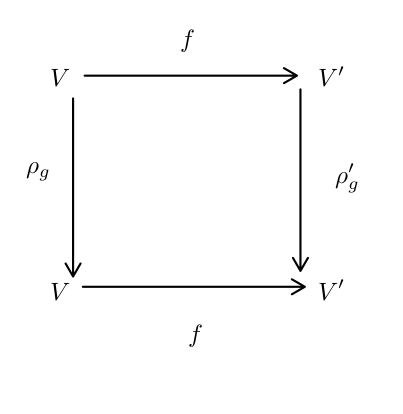
\includegraphics[scale=0.3]{figures/rep-iso2.png}
%  \caption{Représentations linéaires isomorphes.}
%  \label{}
%\end{figure}



%\begin{figure}[h!]
%  \centering
%  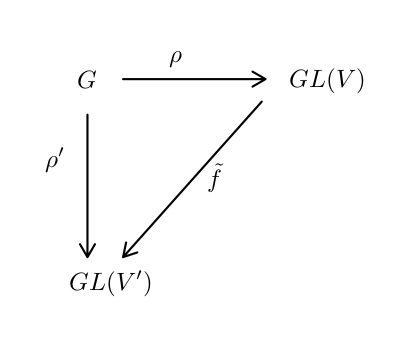
\includegraphics[scale=0.3]{figures/rep-iso.png}
%  \caption{Diagramme commutatif de deux représentations isomorphes.}
%  \label{}
%\end{figure}

\begin{remark}
  Dire que le diagramme ci-dessus commute, c'est dire que

  \[\tilde{f} \circ \rho = \rho'.\]

  D'où, pour tout \(g \in G\), \(\rho'_g = \tilde{f} (\rho_g) = f \circ \rho_g \circ f ^{-1} \), i. e. \( \rho_g' \circ f = f \circ \rho_g\).

  \begin{equation*}
    \xymatrix{
  V\ar[r]^-{f}\ar[d]_-{\rho_g}\ar@{}[rd]|{\circlearrowright}&V'\ar[d]^-{\rho_g'}\\
  V\ar[r]_-{f}&V'
  }
  \end{equation*}
\end{remark}

\begin{remark}
  En termes de matrices, cela signifie  que les matrices associées à la première représentation sont semblable à leurs homologues dans la deuxième, via la même matrice de passage :

  \[\forall g \in G, \operatorname{Mat}(\rho_g') = \operatorname{Mat}(f) \times \operatorname{Mat}(\rho_g) \times \operatorname{Mat}(f) ^{-1}. \]
\end{remark}

\subsection{Sous-représentations}

\begin{definition}
  Si \(\rho : G \to GL(V)\) est une représentation linéaire d'un groupe \(G\) et si \(W\) est un sous-espace vectoriel de \(V\) stable par la représentation (i.e. stable par les automorphismes \(\rho_g\) pour \(g \in G\), i.e. \(\forall g \in G, \rho_g(W) \subset W\), i. e. \(\forall g \in G, \forall w \in W, \rho_g(w) \in W\)), alors cela nous permet de définir une \textbf{sous-représentation}

  \[\begin{matrix}
  \rho _{|W} : & G & \longrightarrow & GL(W) \\
  \ & g & \longmapsto & \left( \rho _{g _{|W}} : \begin{matrix}
  W & \longrightarrow & W \\
  w & \longmapsto & \rho_g(w)
  \end{matrix}\right).
  \end{matrix}\]
\end{definition}

\begin{definition}
  Une représentation \(\rho : G \to GL(V)\) est dite \textbf{irréductible} si les seuls sous-espaces stables de \(V\) sont \(\{0\} \text{ et } V\).
\end{definition}

\begin{remark}
  Les représentations de degré 1 sont bien évidemment des représentations irréductibles.
\end{remark}

\begin{proof}[Démonstration personnelle]
  Soit \(\rho : G \to GL(V)\) une représentation de degré 1. Alors \(\operatorname{dim}(V) = 1\). Si \(W\) sous-espace vectoriel de \(V\), alors
  \begin{enumerate}
    \item \(\operatorname{dim}(W)=0\) et dans ce cas \(W = \{ 0 \} \);
    \item ou bien \(\operatorname{dim}(W)=1\) et dans ce cas \(W = V\).
  \end{enumerate}
\end{proof}

\section{Théorème de Maschke}

On définit tout d'abord la notion de \textbf{somme directe} de représentations. On rappelle que si \(V\) est un espace vectoriel et si \(W, W'\) sont deux sous-espaces vectoriels de \(V\), alors on dit que \(V\) est \textbf{somme directe} de \(W\) et \(W'\) si tout \(x \in V\) peut s'écrire de façon unique sous la forme :

\[x = w+w', \text{ avec } w \in W, w' \in W'. \]

Il revient au même de dire que

\[W \cap W' = \{ 0 \} \text{ et } \operatorname{dim}(V) = \operatorname{dim}(W)+ \operatorname{dim}(W').\]

On écrit alors \(V = W \oplus W'\) et l'on dit que \(W'\) est un \textbf{supplémentaire} de \(W\) dans \(V\).

L'application \(p : \begin{matrix}
  V & \longrightarrow & V \\
  v = \underbrace{w}_{\in W} + \underbrace{w'}_{\in W'} & \longmapsto & w
\end{matrix}\) est alors appelé le \textbf{projecteur} de \(V\) sur \(W\) associé à la décomposition \(V = W \oplus W'\). On a \(\operatorname{Im}(p) = W\) et \(\operatorname{Ker}(p) = W'\) et \(p(x) = x\) si \(x \in W\).

Réciproquement, si \(p\) est une application linéaire de \(V\) sur lui-même vérifiant ces deux propriétés, on vérifie que \(V = W \oplus \operatorname{Ker}(p)\), avec \(\operatorname{Ker}(p) = \{ v \in V, p(v) = 0 \} \). On établit ainsi une \textbf{bijection} entre les projecteurs de \(V\) sur \(W\) et les \textbf{supplémentaires} de \(W\) dans \(V\).

\begin{definition}
  Soient \(\rho : G \longrightarrow GL(V) \text{ et } \rho' : G \longrightarrow GL(V')\) deux représentations d'un groupe \(G\). On définit la somme directe \(\rho \oplus \rho'\) comme étant la représentation d'espace vectoriel \(V \oplus V'\) définie par

  \[\begin{matrix}
  \rho \oplus \rho' : & G & \longrightarrow & GL(V \oplus V') \\
  \ & g & \longmapsto & \left( (\rho \oplus \rho')_g  : \begin{matrix}
  V \oplus V' & \longrightarrow & V \oplus V' \\
  v + v' & \longmapsto & \rho_g(v) + \rho_g'(v')
  \end{matrix}\right).
  \end{matrix}\]
\end{definition}

\begin{thm}[De Maschke]\label{Maschke}
  Toute représentation linéaire complexe de dimension finie d'un groupe fini est \textbf{somme directe de représentations irréductibles}.
\end{thm}

\begin{lemma}\label{lemme-maschke}
  Tout sous-espace stable d'une représentation linéaire complexe de degré fini d'un groupe fini admet un sous-espace \textbf{supplémentaire \emph{stable}}.
\end{lemma}

\begin{remark}
  {\fontencoding{U}\fontfamily{futs}\selectfont\char 66\relax} Il existe un produit scalaire hermitien sur l'espace de la représentation qui est stable par l'action du groupe. En effet, si \(\langle \cdot, \cdot \rangle \) désigne un produit scalaire quelconque sur \(V\), le produit suivant est stable par \(\rho\) :

  \[\forall x, y \in V, \langle x, y \rangle_{\rho} := \frac{1}{\lvert G \rvert} \sum_{g \in G}^{} \langle \rho_g(x), \rho_g(y) \rangle. \]

  En effet, si \(h \in G\), alors on a:

  \begin{gather*}
    \langle \rho_h(x), \rho_h(y) \rangle _{\rho} = \frac{1}{\lvert G \rvert} \sum_{g \in G}^{} \langle \rho_g(\rho_h(x)), \rho_g (\rho_h(y)) \rangle  \\
    = \frac{1}{\lvert G \rvert} \sum_{g \in G}^{} \langle \rho _{gh}(x), \rho _{gh}(y) \rangle  = \langle x, y \rangle _{\rho},
  \end{gather*}

  car \(g \longmapsto gh\) est une bijection de \(G\) sur lui-même.
\end{remark}


\begin{proof}[Démonstration du lemme \ref{lemme-maschke}]
  Si \(W\) est un sous-espace vectoriel de \(V\) stable sous l'action de \(G\), alors le supplémentaire \textbf{orthogonal} de \(W\) est lui aussi stable sous l'action puisque : \(W \subset V\) stable sous l'action de \(G\) par \(\rho\), i. e. \( \forall g \in G, \rho_g(W) \subset W\). On a

  \[W ^{\perp} := \{  x \in V \mid \langle x, w \rangle _{\rho} = 0,  \forall w \in W \}.\]

  Montrons que \( W ^{\perp}\) est stable par \(\rho\). Soit \(g \in G\), soit \(x \in W ^{\perp}\), montrons que \(\rho_g(x) \in W ^{\perp}\). Soit \(w \in W\), montrons que \(\langle \rho_g(x), w \rangle _{\rho}=0\). On a

  \begin{gather*}
    \langle \rho_g(x), w \rangle_{\rho} = \langle \rho _{g ^{-1} }(\rho_g(x)), \rho _{g ^{-1} }(w) \rangle _{\rho} = \langle x, \rho _{g ^{-1} (w)} \rangle _{\rho} = 0,
  \end{gather*}

  car \(\rho _{g ^{-1} }(w) \in W\).
\end{proof}

\begin{proof}[Démonstration du théorème \ref{Maschke}]
  Si \(\operatorname{dim}(V)=1\) ou si \(V\) est irréductible, c'est démontré.

  Si \(\operatorname{dim}(V) \geq 2\) et \(V\) est non irréductible, alors \(V\) possède une sous-représentation \(W\) distincte de \(\{ 0 \} \) et \(V\). Si \(\langle \cdot, \cdot \rangle _{\rho}\) est un produit scalaire hermitien sur \(V\) invariant sous l'action de \(G\), le supplémentaire orthogonal \(W ^{\perp}\) de \(W\) est lui aussi stable par \(G\). On a alors \(V = W \oplus W'\) et \(W\) et \(W'\) sont de dimensions inférieures à celle de \(V\).

  Par l'hypothèse de récurrence, on peut les décomposer en sommes directes de représentations irréductibles.
\end{proof}

\section{Caractère d'une représentation}

\begin{definition}
  On appelle \textbf{caractère} de la représentation \(\rho : G \longrightarrow GL(V)\) l'application

  \[\begin{matrix}
  \chi_{\rho} : & G & \longrightarrow & \mathbb{C} \\
  \ & g & \longmapsto & \chi_{\rho}(g) := \operatorname{Tr}(\rho_g).
  \end{matrix}\]

  où \(\operatorname{Tr}(\rho_g)\) désigne la \textbf{trace} de l'endomorphisme \(\rho_g\).

  Le degré du caractère \(\chi_\rho\) est défini comme le degré de la représentation \(\rho\).
\end{definition}

\begin{prop}[Propriétés du caractère d'une représentation]
  Soit \(\rho: G \longrightarrow GL(V)\) une représentation d'un groupe fini \(G\) de caractère \(\chi _{\rho}\).

  \begin{enumerate}
    \item \(\chi_{\rho}(e) = \operatorname{dim}(V) = \text{degré de } \rho = \text{degré de } \chi _{\rho}\).
    \item \(\forall g \in G, \chi _{\rho}(g ^{-1}) = \overline{\chi _{\rho}(g)}\) (conjugaison complexe).
    \item \(\forall g, h \in G\), \(\chi _{\rho}(g h g ^{-1} ) = \chi _{\rho}(h)\), i. e. \(\chi _{\rho}\) est une \textbf{fonction centrale} sur \(G\), i. e. \(\chi _{\rho}\) est \textbf{constante sur les classes de conjugaison}.
    \item \(\chi _{\rho\oplus \rho'} = \chi _{\rho}+ \chi _{\rho'}\), si \(\rho' : G \longrightarrow GL(V')\) est une représentation de \(G\).
    \item Si \(\rho, \rho'\) sont équivalentes, alors \(\chi _{\rho} = \chi _{\rho'}\).
  \end{enumerate}
\end{prop}



\begin{proof}\marginnote{27-09-2023}

  \
  Soit \(\rho : G \longrightarrow GL(V)\) représentation linéaire d'un groupe fini \(G\) de caractère \(\chi _{\rho}\).
  \begin{enumerate}
    \item Par définition, \(\chi _{\rho}(e) = \operatorname{Tr}(\rho_e) \). Puisque \(\rho\) est un morphisme de groupes, l'image de l'élément neutre de \(G\) par \(\rho\) est donc l'élément neutre de \(GL(V)\), à savoir l'identité \(\operatorname{id}_V\) sur \(V\). D'où : \[\chi _{\rho}(e) = \operatorname{Tr}(\rho_e) = \operatorname{Tr}(id_V) = \operatorname{Tr}(I _{\operatorname{dim}(V)}). \]

    C'est la matrice identité à \(\operatorname{dim}(V)\) lignes et \(\operatorname{dim}(V)\) colonnes.

    \item Montrons que \(\forall g \in G, \chi _{\rho}(g ^{-1} ) = \overline{\chi _{\rho}(g)}\).

    Remarquons que si \(G\) est fini et si \(g \in G\), alors les valeurs propres de \(\rho_g\) (les racines du polynôme de cet endomorphisme) sont les racines de l'unité. En effet, si \(G\) est d'ordre \(n\), alors, par le théorème de Lagrange, on a \(g ^{n} = e\). D'où

    \[\rho_g ^{n} = \rho _{g ^{n}} = \rho_e = \operatorname{id}_V,\]

    donc le polynôme minimal de \(\rho_g\) divise \(X ^{n}-1\). Or les racines du polynôme minimal de \(\rho_g\) sont les valeurs propres de \(\rho_g\). Donc les valeurs propres de \(\rho_g\) sont les racines de l'unité.

    En particulier, les valeurs propres de \(\rho_g\) sont des nombres complexes de module 1. Donc, si \(\lambda \) est une valeur propre de \(\rho_g\), alors \(\lvert \lambda  \rvert = 1\) et donc \(\lambda  ^{-1} = \overline{\lambda }\). De plus, les valeurs propres de \(\rho _{g ^{-1}} = \rho _{g} ^{-1} \) (car \(\rho\) est un morphisme) sont les inverses de celles de \(\rho_g\).

    En effet, si \(f(x) = \lambda x\) avec \(x\) non nul et \(f \in GL(V)\), alors

    \[x =  f ^{-1} (f(x)) = f ^{-1} (\lambda x) = \lambda f ^{-1} (x),\]

    d'où \(f ^{-1} (x) = \lambda ^{-1} (x)\) et donc \(x\) est vecteur propre de \(f ^{-1} \) pour la valeur propre \(\lambda ^{-1} \).

    Enfin, puisque la trace d'un endomorphisme est la somme de ses valeurs propres (comptées avec leur multiplicités), on en déduit que

    \[\chi _{\rho}(g ^{-1}) = \overline{\chi _{\rho}(g)}. \]

    \item Soient \(g, h \in G\). On a

    \begin{gather*}
      \chi _{\rho}(g h g ^{-1}) \stackrel{\text{déf}}{=} \operatorname{Tr}(\rho _{ghg ^{-1}}) \stackrel{\text{morphisme}}{=} \operatorname{Tr}(\rho_g \circ \rho_h \circ \rho _{g ^{-1}}) \\
      = \operatorname{Tr}(\rho_g \circ \rho_h \circ \rho_g ^{-1}) \stackrel{\operatorname{Tr}(AB) = \operatorname{Tr}(BA)}{=} \operatorname{Tr}(\rho_g ^{-1} \circ \rho_g \circ \rho_h) = \operatorname{Tr}(\rho_h) = \chi _{\rho}(h).
    \end{gather*}

    Donc \(\chi _{\rho}\) est une fonction centrale sur \(G\), i. e. qu'elle prend les mêmes valeurs sur les éléments d'une même classe de conjugaison.

    \item Soient \(\rho : G \longrightarrow GL(V)\) et \(\rho' : G \longrightarrow GL(V')\) deux représentations de \(G\). La somme directe de \(\rho\) et \(\rho'\) est la représentation
     \[\begin{matrix}
      \rho \oplus \rho' : & G & \longrightarrow & GL(V \oplus V') \\
      \ & g & \longmapsto & \left( (\rho \oplus \rho')_g  : \begin{matrix}
      V \oplus V' & \longrightarrow & V \oplus V' \\
      v + v' & \longmapsto & \rho_g(v) + \rho_g'(v')
      \end{matrix}\right).
      \end{matrix}\]

      Si \((e_1, \dots, e_n)\) est une base de \(V\) et \((e_1', \dots, e_m')\) est une base de \(V'\), alors

      \[B = (e_1+0, \dots, e_n+0, 0 + e_1', \dots, 0 + e_m')\]

      est une base de \(V \oplus V'\).

      D'où

      \[\operatorname{Mat}_B((\rho \oplus \rho')_g) = \begin{pmatrix}
      \operatorname{Mat} _{(e_1, \dots, e_n)}(\rho_g) & 0 \\
      0 & \operatorname{Mat} _{(e_1', \dots, e_m')}(\rho_g')
      \end{pmatrix}, \]

      d'où

      \begin{gather*}
        \chi _{(\rho\oplus \rho')_g} = \operatorname{Tr}((\rho\oplus \rho')_g) = Tr(\operatorname{Mat}_B((\rho \oplus \rho')_g))\\
         = \operatorname{Tr}(\operatorname{Mat} _{(e_1, \dots, e_n)}(\rho_g))+ \operatorname{Tr}(\operatorname{Mat} _{(e_1', \dots, e_m')}(\rho_g')) = \chi _{\rho}(g) + \chi _{\rho'}(g').
      \end{gather*}

      \item Soient \(\rho : G \longrightarrow GL(V)\) et \(\rho' : G \longrightarrow GL(V')\) deux représentations équivalentes de \(G\). Alors il existe une isomorphisme \(f : V \longrightarrow V'\) tel que

      \[\forall g \in G, \rho_g' = f \circ \rho_g \circ f ^{-1}.\]

      D'où, pour tout \(g \in G\), on a

      \[\chi _{\rho'}(g) = \operatorname{Tr}(\rho_g') = \operatorname{Tr}(f \circ \rho_g \circ f ^{-1}) = \operatorname{Tr}(\rho_g) = \chi _{\rho}(g).\]

      Donc \(\chi _{\rho} = \chi _{\rho'}\).
  \end{enumerate}
\end{proof}

%\paragraph{Exemples de calcul de caractères}

\begin{exemple}[Calcul de caractères]

  \

  \begin{enumerate}
    \item Si \(G\) opère sur un ensemble fini \(X\), considérons la représentation de permutations \(\rho\) associée, avec \(V = \bigoplus _{x \in X} \langle e_x \rangle = \bigoplus _{x \in X} \mathbb{C} e_x\).

    \[\begin{matrix}
    \rho : & G & \longrightarrow & GL(V) \\
    \ & g & \longmapsto &\left( \rho_g : \begin{matrix}
    V & \longrightarrow & V \\
    \varepsilon_x & \longmapsto & \rho_g(\varepsilon_x) := \varepsilon _{g \cdot x}
    \end{matrix} \right).
    \end{matrix}\]

    On a \(\chi _{\rho} : G \longrightarrow \mathbb{C}\) tel que \(\chi _{\rho}(g) = \operatorname{Tr}(\rho_g)\). Dans une base \((e_x) _{x \in X}\) de \(V\), pour \(g \in G\) fixé, la matrice de \(\rho_g\) est une matrice de permutations, i.e. a exactement un 1 par ligne et par colonne et tous les autres coefficients sont nuls.

    De plus, si \(\operatorname{Mat} _{(e_x)} (\rho_g) = (a _{ij}) _{i,j}\), alors le terme diagonal correspondant à \(\rho_g(e_x)\) sera égal à 1 si et seulement si \(g \cdot x = x\) si et seulement si \(x\) est un point fixe de \(g\). Sinon il vaudra 0. Donc

    \[\chi _{\rho}(g) = \operatorname{Tr}(\rho_g) = \sharp \{ x \in X \mid g \cdot x = x \}.\]

    \item \emph{Caractère de la représentation régulière (c'est le cas particulier de la représentation de permutations \(\rho\) avec \(G\) fini, \(X = G\), l'action étant la multiplication dans \(G\)).}

    On a alors, pour tout \(g \in G\) :

    \begin{gather}
      \chi _{\rho}(g) = \operatorname{Tr}(\rho_g) = \sharp \{ x \in G \mid g x=x \} = \begin{cases}
        \lvert G \rvert \text{ si } g=e \\
        0 \text{ si } g \neq e.
      \end{cases}
    \end{gather}
  \end{enumerate}
\end{exemple}


\begin{definition}
  Un caractère d'un groupe \(G\) est dit \textbf{irréductible} si c'est le caractère d'une représentation irréductible de \(G\).
\end{definition}

\section{Orthogonalité des caractères irréductibles}

Soit \(G\) un groupe fini. On considère le \(\mathbb{C}\)-espace vectoriel \(\mathscr{F}(G) \) des fonctions définies sur \(G\) et à valeurs dans \(\mathbb{C}\). On munit le \(\mathbb{C}\)-espace vectoriel \(\mathscr{F}(G)\) d'une structure hermitienne donnée par le produit scalaire suivant : pour \(\varphi, \psi \in \mathscr{F}(G)\), on a

\[\langle \varphi, \psi \rangle := \frac{1}{\lvert G \rvert} \sum_{g \in G}^{} \overline{\varphi(g)} \psi(g).\]

\begin{remark}
  Si \(f \in \mathscr{F}(G) \), alors \[f = \sum_{g \in G}^{} \lambda \operatorname{Ind}_g = \sum_{g \in G}^{} f(g) \operatorname{Ind}_g, \]

  où

  \[\begin{matrix}
  \operatorname{Ind}_g : & G & \longrightarrow & \mathbb{C} \\
  \ & x & \longmapsto & \begin{cases}
    1 \text{ si } x=g \\
    0 \text{ sinon. }
  \end{cases}
  \end{matrix}\]

  Donc \((\operatorname{Ind}_g) _{g \in G}\) est une base de \(\mathscr{F}(G)\). En particulier, \(\operatorname{dim} _{\mathbb{C}}(\mathscr{F}(G)) = \lvert G \rvert\).
\end{remark}

\begin{lemma}[De Schur]\label{schur}
  Soit \(\rho : G \longrightarrow GL(V)\) et \( \rho' : G \longrightarrow GL(V')\) deux représentations linéaires irréductibles d'un groupe fini \(G\). Soit \(f : V \longrightarrow V'\) une application linéaire vérifiant :

  \[\forall g \in G, f \circ \rho_g = \rho_g' \circ f.\]

  \begin{enumerate}
    \item Si \(\rho \text{ et }  \rho'\) ne sont pas isomorphes, alors \(f = 0\).
    \item Si \(\rho \text{ et } \rho'\) sont isomorphes, alors \(f\) est une homothétie.
  \end{enumerate}
\end{lemma}

\begin{proof}

  \

  \begin{enumerate}
    \item Montrons la contraposée : on suppose que \(f\) n'est pas l'application nulle.

    Le sous-espace \(\operatorname{Ker}(f)\) de \(V\) est stable par \(\rho\). En effet, si \(g \in G\) et si \(x \in \operatorname{Ker}(f)\), alors \(\rho_g(x) \in \operatorname{Ker}(f)\), car :

    \begin{gather*}
      f(\rho_g(x)) = (f \circ \rho_g)(x) = (\rho_g' \circ f)(x) = \rho_g'(f(x)) = \rho_g'(0) = \rho_g'(0)=0.
    \end{gather*}

    Comme \(f \neq 0\), i. e. \(\operatorname{Ker}(f) \neq V\), on en déduit que \(\operatorname{Ker}(f) = \{ 0 \}\) par irréductibilité de \(\rho\).

    De même, le sous-espace \(\operatorname{Im}(f)\) de \(V'\) est stable par \(\rho'\). En effet, si \(g \in G\) et \(y=f(x) \in \operatorname{Im}(f)\), alors \(\rho_g'(y) \in \operatorname{Im}(f)\), car

    \begin{gather*}
      \rho_g'(y) = \rho_g'(f(x)) = (\rho_g' \circ f)(x) = (f \circ \rho_g)(x) = f(\rho_g(x)).
    \end{gather*}

    Puisque \(f \neq 0\) (i. e. \(\operatorname{Im}(f) \neq \{ 0 \} \)), on en déduit que \(\operatorname{Im}(f) = V'\) par irréductibilité de \(\rho'\).

    En conclusion, \(f\) est bijective. Donc \(f\) est un isomorphisme et donc \(\rho\) et \(\rho'\) sont deux représentations isomorphes.

    \item On suppose que \(\rho : G \longrightarrow GL(V)\) et \(\rho' : G \longrightarrow GL(V')\). On peut donc identifier \(V\) et \(V'\) (et \(\rho \text{ et } \rho'\)). Puisque \(\mathbb{C}\) est algébriquement clos (théorème de d'Alembert-Gauss), l'endomorphisme \(f : V \longrightarrow V \) admet une valeur propre \(\lambda \in \mathbb{C}\). Le sous-espace propre \(\operatorname{SEP}(f, \lambda)\) de \(f\) pour la valeur propre \(\lambda\) est stable par \(\rho\).

    En effet, si \(g \in G\) et si \(x \in \operatorname{SEP}(x, \lambda)\), alors \(\rho_g(x) \in \operatorname{SEP}(f, \lambda)\), car \[f(\rho_g)(x) = \rho_g(f(x)) = \rho_g(\lambda x) = \lambda \rho_g(x).\]

    Donc \( \underbrace{\operatorname{SEP}(f, \lambda)}_{\neq \{ 0 \}} = V\) par irréductibilité de \(\rho\). D'où, \( \forall x \in V, f(x) = \lambda x\), i. e. \(f\) est une homothétie de rapport \(\lambda\).
  \end{enumerate}
\end{proof}

\begin{prop}\label{syst-orth}
  Les caractères irréductibles d'un groupe \(G\) forment un système orthonormal de fonctions de l'espace vectoriel hermitien \(\mathscr{F}(G) \), i. e.

  \[\langle \chi, \chi' \rangle = \begin{cases}
    1 \text{ si } \chi = \chi' \\
    0 \text{ sinon,  }
  \end{cases} \]

  si \(\chi, \chi'\) ne sont pas des caractères irréductibles de \(G\).
\end{prop}

\begin{proof}
  Soient \(\rho : G \longrightarrow GL(V)\) et \(\rho' : G \longrightarrow GL(V')\) deux représentations irréductibles de \(G\) et soient \(\chi \text{ et } \chi'\) leurs caractères associés.

  Soit \(g \in G\), notons \(\operatorname{Mat}(\rho_g) = (a _{ij}(g)) _{1 \leq i, j \leq d}, \operatorname{Mat}(\rho_g') = (a _{ij}'(g)) _{1 \leq i, j \leq d'}\), où \(d = \operatorname{deg}(\chi) = \operatorname{dim}(V)\) et \(d' = \operatorname{deg}(\chi') = \operatorname{dim}(V')\). On a :

  \begin{gather*}
    \chi(g) = \operatorname{Tr}(\rho_g) = \sum_{i=1}^{d} a _{ii}(g) \text{ et } \chi'(g) = \sum_{i=1}^{d'}a _{ii}'(g).
  \end{gather*}

  D'où

  \begin{gather*}
    \langle \chi, \chi' \rangle = \frac{1}{\lvert G \rvert} \sum_{g \in G} \overline{\chi(g)} \chi'(g) = \frac{1}{\lvert G \rvert} \sum_{g \in G}^{} \sum_{i,j}^{} \overline{a _{ii}(g)} a _{ii}'(g)= \begin{cases}
      0 \text{ si }  \rho \text{ et } \rho' \text{ non isomorphes, } \\
      1 \text{ si }  \rho \text{ et } \rho' \text{ son isomorphes. }
    \end{cases}
  \end{gather*}
\end{proof}



\begin{exo}\marginnote{03-10-2023}
  On note \(\hat{G}\) l'ensemble des caractères linéaires d'un groupe \(G\), i. e. l'ensemble des morphismes \(\chi : G \longrightarrow \mathbb{C} ^{*}\) (ce sont les caractères des représentations de degré 1 (donc irréductibles) de \(G\)). On définit le produit \(\chi\chi'\) de deux caractères linéaires de \(G\) : pour \(g \in G\),

  \[(\chi \chi')(g) = \chi(g)\chi'(g).\]

  \begin{enumerate}
    \item Montrer que \(\hat{G}\), muni  de ce produit, est un groupe abélien.
    \item On rappelle que le caractère trivial  est défini par :
    \[\begin{matrix}
    \chi_0 : & G & \longrightarrow & \mathbb{C} ^{*} \\
    \ & g & \longmapsto & 1.
    \end{matrix}\]

    Montrer que si \(G\) est fini et si \(\chi \in \hat{G}\), alors

    \[\frac{1}{\lvert G \rvert} \sum_{g \in G}^{} \chi(g) = \begin{cases}
      1 \text{ si } \chi = \chi_0 \\
      0 \text{ sinon. }
    \end{cases}\]

    \item En déduire les relations d'orthogonalité des caractères linéaires : si \(\chi, \chi' \in \hat{G}\), alors

    \begin{gather*}
      \langle \chi, \chi' \rangle = \frac{1}{\lvert G \rvert} \sum_{g \in G}^{}  \overline{\chi(g)} \chi'(g) = \begin{cases}
        1 \text{ si } \chi = \chi' \\
        0 \text{ sinon. }
      \end{cases}
    \end{gather*}
  \end{enumerate}

  \end{exo}

  \begin{proof}

    \

  \begin{enumerate}
    \item \begin{itemize}
      \item[$\star$] Le produit est bien une loi de composition interne dans \(\hat{G}\) car si \(\chi, \chi' \in \hat{G}\), alors \(\chi \chi' : G \longrightarrow \mathbb{C} ^{*}\) est bien un morphisme de groupes.

      En effet, si \(g, g' \in G\), alors

      \begin{gather*}
        (\chi \chi')(gg') = \chi(gg') \chi'(gg') = \chi(g)\chi(g') \chi'(g)\chi'(g') = (\chi(g) \chi'(g))(\chi(g')\chi'(g')) = (\chi\chi')(g)(\chi\chi')(g').
      \end{gather*}

      \item[$\star$] La loi est associative, car la multiplication l'est dans \(\mathbb{C}\).
      \item[$\star$] L'application \(\chi _{0} : \begin{matrix}
      G & \longrightarrow & \mathbb{C} ^{*} \\
      g & \longmapsto & 1
      \end{matrix}\) est bien un morphisme de groupes et est l'élément neutre de \(\hat{G}\).

      \item[$\star$] Si \(\chi \in \hat{G}\), alors le caractère linéaire \(\chi' : G \longrightarrow \mathbb{C} ^{*}\) défini par \[\chi'(g) = \frac{1}{\chi(g)} = (\chi'(g)) ^{-1} = \chi(g ^{-1})\]

      vérifie \(\chi \chi' = \chi _{0} = \chi'\chi\), et donc \(\chi ^{-1} = \chi'\) est le symétrique de \(\chi\) dans \(\hat{G} \), car \(\chi ^{-1}\) est encore un morphisme de groupes. En effet, si \(g, g' \in G\), alors

      \[\chi ^{-1}(gg') = \chi((gg') ^{-1}) = \chi ((g')^{-1} g ^{-1}) = \chi((g')^{-1}) \chi(g ^{-1}) = \chi ^{-1}(g') \chi ^{-1}(g) = \chi ^{-1}(g) \chi ^{-1}(g').\]

      De plus, \(\chi \chi' = \chi' \chi, \forall \chi, \chi' \in \hat{G}\), c'est-à-dire \(\hat{G}\) est un groupe abélien.
    \end{itemize}

    \item Si \(\chi = \chi_0\), alors

    \[\frac{1}{\lvert G \rvert} \sum_{g \in G}^{} \chi_0(g) = \frac{1}{\lvert G \rvert} \sum_{g \in G}^{} 1 = 1.\]

    Soit maintenant \(\chi \in \hat{G}\) tel que \(\chi \neq \chi_0\). Il existe alors \(a \in G\) tel que \(\chi(a) \neq 1\). On a :

    \begin{gather*}
      \frac{\chi(a)}{\lvert G \rvert} \sum_{g \in G}^{} \chi(g) = \frac{1}{\lvert G \rvert} \sum_{g \in G}^{} \chi(a) \chi(g) = \frac{1}{\lvert G \rvert}\sum_{g \in G}^{}  \chi(ag)= \frac{1}{\lvert G \rvert} \sum_{g \in G}^{} \chi(g),
    \end{gather*}

    car l'application \(f_a\) définie par \(f_a : \begin{matrix}
    G & \longrightarrow & G \\
    g & \longmapsto & ag
    \end{matrix}\) est une bijection. D'où :

    \begin{gather*}
      (\chi(a) - 1) \left(\frac{1}{\lvert G \rvert} \sum_{g \in G}^{} \chi(g) \right) = 0.
    \end{gather*}

    Cette égalité a lieu dans \(\mathbb{C}\) qui est un corps, donc en particulier un anneau intègre et donc ne contient pas de diviseurs de 0. Or \(\chi(a) -1 \neq 0\), car \(\chi(a) \neq 1\). Donc

    \[\frac{1}{\lvert G \rvert}\sum_{g \in G}^{} \chi(g) = 0.\]

    \item Si \(\chi \in \hat{G}\), alors on a :

    \begin{gather*}
      \langle \chi, \chi \rangle  = \frac{1}{\lvert G \rvert} \sum_{g \in G} \overline{\chi(g)} \chi(g) = \frac{1}{\lvert G \rvert} \sum_{g \in G} \frac{1}{\chi(g)} \chi(g),
    \end{gather*}

    car, \(G\) étant fini, on a pour tout \(g \in G\), \(g ^{\lvert G \rvert} = e\) (par le théorème de Lagrange) et donc \(\chi(g ^{\lvert G \rvert})= \chi(g) ^{\lvert G \rvert}\), donc \(\chi(g)\) est une racine de l'unité dans \(\mathbb{C}\) ! En particulier, \(\chi(g)\) est un nombre complexe de module 1, et donc son conjugué est égal à son inverse

    \[\overline{\chi(g)} = \frac{1}{\chi(g)}.\]

    Donc \(\langle \chi, \chi' \rangle = \frac{1}{\lvert G \rvert} \sum_{g \in G} 1 = \frac{\lvert G \rvert}{\lvert G \rvert}=1. \)

    \

    Soient \(\chi, \chi' \in \hat{G}\) tels que \(\chi \neq \chi'\). Il existe donc \(a \in G\) tel que \(\chi(a) \neq \chi'(a)\). On a :

    \begin{gather*}
      \langle \chi, \chi' \rangle  = \frac{1}{\lvert G \rvert} \sum_{g \in G}^{} \overline{\chi(g)} \chi'(g) = \frac{1}{\lvert G \rvert} \sum_{g \in G} \overline{\chi(ag)} \chi'(ag)
    \end{gather*}

    grâce au même argument que dans la question précédente. D'où

    \begin{gather*}
      \langle \chi, \chi' \rangle = \frac{1}{\lvert G \rvert} \sum_{g \in G} \chi(a)\chi(g) \chi'(a)\chi'(g) \\
       = \frac{\overline{\chi(a)} \chi'(a)}{\lvert G \rvert} \sum_{g \in G}^{} \overline{\chi(g)} \chi'(g)  = \overline{\chi(a)} \chi'(a) \langle \chi, \chi' \rangle,
    \end{gather*}

    d'où \((\overline{\chi(a)} \chi'(a) - 1) \langle \chi, \chi' \rangle = 0\). On a donc \(\overline{\chi(a)} \chi'(a) - 1 = 0\) ou \(\langle \chi, \chi' \rangle = 0\). Or \(\overline{\chi(a)}\chi'(a) = 1 \iff \chi'(a) = \frac{1}{\overline{\chi}(a)} = \chi(a)\). Or on a \(\chi'(a) \neq \chi(a)\). Donc \(\langle \chi, \chi' \rangle = 0\).
  \end{enumerate}
\end{proof}

\section{Théorème de Frobenius}

Soit \(G\) un groupe et soit \(\mathscr{F}(G) = \{ \text{fonctions } f : G \longrightarrow \mathbb{C} \} \) l'ensemble des fonctions définies sur \(G\) à valeurs dans \(\mathbb{C}\). Les fonctions \(\mathscr{F}(G)\) qui sont \textbf{constantes} sur  \textbf{les classes de conjugaison} de \(G\) sont appelées fonctions \textbf{centrales} sur \(G\). On note \(\mathscr{F}_C(G)\) l'ensemble des fonctions centrales :

\[\mathscr{F}_C(G) := \{ f : G \longrightarrow \mathbb{C} ^{*}, \forall g, h \in G, f (ghg ^{-1}) = f(h)\}.\]

On a vu que les caractères \(\chi _{\rho}\) des représentations \(\rho\) de \(G\) sont des fonctions centrales sur \(G\). \(\mathscr{F}_C(G)\) est un sous-espace vectoriel de \(\mathscr{F}(G)\).

\begin{thm}[De Frobenius]
  Les caractères \textbf{irréductibles} d'un groupe \(G\) forment une \textbf{base orthonormale} de l'espace \(\mathscr{F}_C(G)\) de fonctions centrales sur \(G\).
\end{thm}

\begin{proof}[Sketch of proof]
  On a déjà vu que les caractères irréductibles forment un système libre de fonctions de \(\mathscr{F}_C(G)\) (proposition \ref{syst-orth}). Notons \(F\) le sous-espace vectoriel engendré par les caractères irréductibles de \(G\). L'idée de la preuve est de vérifier que l'orthogonal  \(F ^{\perp}\) de \(F\) est réduit à 0 en utilisant de lemme de Schur (cf \ref{schur}).
\end{proof}

\begin{corollary}\label{nb-cl-iso}
  Le nombre de (classes d'isomorphismes de) représentations irréductibles d'un groupe \(G\) est égal au nombre de classes de conjugaison de \(G\).
\end{corollary}

\begin{proof}
  D'après le théorème de Frobenius, le nombre de représentations irréductibles d'un groupe \(G\) est égal à la dimension de l'espace vectoriel \(\mathscr{F}_C(G)\) des fonctions centrales sur \(G\). Or une fonction est centrale si et seulement si elle est constante sur chaque classe de conjugaison ; une fonction centrale \(\phi : G \longrightarrow \mathbb{C}\) peut donc s'écrire de manière unique sous la forme :

  \[\phi = \sum_{C \in \operatorname{Conj}(G)} \lambda_C 1 _{C}, \]

  où \(\operatorname{Conj}(G)\) est l'ensemble de classes de conjugaison de \(G\) et \(1 _{C}\) est la fonction indicatrice de \(C\), i. e. \(1_C(g) = \begin{cases}
    1 \text{ si } g \in C\\
    0 \text{ sinon }
  \end{cases}\) et où \(\lambda_C \in \mathbb{C}\) (on a \(\lambda_C = \phi(g)\) où \(g\) est n'importe quel élément de \(C\)). Les fonctions indicatrices \(1_C\), pour \( C \in \operatorname{Conj}(G)\), forment donc une base de \(\mathscr{F}_C(G)\), qui, de ce fait, est de dimension le cardinal de \(\operatorname{Conj}(G)\).
\end{proof}



\begin{remark}[Notation]\marginnote{04-10-2023}
  Si \(G\) est un groupe fini, on note \(\operatorname{Irr}(G)\) l'ensemble des (classes d'isomorphismes de) représentations irréductibles de \(G\) qu'on identifie parfois à l'espace de ces représentations irréductibles.

  \begin{gather*}
    \operatorname{Irr}(G) = \{ \rho : G \longrightarrow W, \text{ représentations irréductibles de } G \text{ à isomorphisme près } \}\\
     = \{ \mathbb{C}-\text{espaces vectoriels } W, \text{ espaces des représentations irréductibles de } G \}.
  \end{gather*}
\end{remark}

\begin{corollary}[Décomposition canonique d'une représentation]\label{cor2}
  Si \(\rho : G \longrightarrow GL(V)\) est une représentation de \(G\), et si \(V = W_1 \oplus \dots \oplus W_k\) est une décomposition de \(V\) en somme directe de représentations irréductibles de \(G\) (i. e. \(\rho = \rho_1 \oplus \dots \oplus \rho_k : G \longrightarrow GL(W_1 \oplus \dots \oplus W_k)\), avec \(\rho_i : G \longrightarrow GL(W_i)\) représentation irréductible pour \(i \in \{ 1, \dots, k \}\)) et si \(W \in \operatorname{Irr}(G)\), alors le nombre \(m_W\) de \(W_i\) qui sont isomorphes à \(W\) (i. e. l'ordre de multiplicité de \(W\) dans cette représentation) est égal à \(\langle \chi_W, \chi_V \rangle \) où \(\chi_W\) et \(\chi_V\) sont les caractères associés aux représentations de \(G\) d'espaces \(W\) et \(V\).

  En particulier, il ne dépend de la décomposition et \[V \simeq \bigoplus _{W \in \operatorname{Irr}(G)} \langle \chi_W, \chi_V \rangle W.\]
\end{corollary}

\begin{proof}
  On a

  \begin{gather*}
    \chi_V = \chi _{W_1} + \dots + \chi _{W_k}.
  \end{gather*}

  D'où

  \begin{gather*}
    \langle \chi _{W}, \chi_V \rangle = \langle \chi_W, \chi _{W_1} \rangle + \dots + \langle \chi_W, \chi _{W_k} \rangle.
  \end{gather*}

  Or \(\langle \chi_W, \chi _{W_i} \rangle = \begin{cases}
    1 \text{ si } W_i \simeq W \\
    0 \text{ sinon. }
  \end{cases} \)

  Donc \(\langle \chi_W, \chi_V \rangle = m_W\).
\end{proof}

\begin{corollary}[Les caractères caractérisent les représentations]
  Deux représentations d'un même groupe fini sont isomorphes si et seulement si elles ont même caractère.
\end{corollary}

\begin{proof}
  D'après le corollaire \ref{cor2}, si \(\rho : G \longrightarrow GL(V)\) et \(\rho' : G \longrightarrow GL(V')\) sont deux représentations de \(G\) ayant même caractère \(\chi\) alors \(V\) et \(V'\) sont tous les deux isomorphes à :

  \[\bigoplus _{W \in \operatorname{Irr}(G)} \langle \chi_W, \chi \rangle W.\]

  Réciproquement, si \(\rho\) et \(\rho'\) sont isomorphes, alors \(\chi _{\rho} = \chi _{\rho'}\) (déjà vu).
\end{proof}

\begin{corollary}[Critère d'irréductibilité]
  Une représentation \(\rho : G \longrightarrow GL(V)\) d'un groupe \(G\) est irréductible si et seulement si \(\langle \chi, \chi \rangle = 1 \) où \(\chi\) est le caractère de \(\rho\).
\end{corollary}

\begin{proof}
  Si \(V \simeq \bigoplus _{W \in \operatorname{Irr}(G)} m_W W\), alors

  \begin{gather*}
    \langle \chi_V, \chi_V \rangle = \left\langle \sum_{w \in \operatorname{Irr}(G)}^{} m_W \chi_W, \sum_{w \in \operatorname{Irr}(G)}^{} m_W \chi_W \right\rangle = \sum_{w \in \operatorname{Irr}(G)}^{} m_W ^2,
  \end{gather*}

  car les caractères irréductibles de \(G\) forment une base orthonormale de l'espace vectoriel des fonctions centrales sur \(G\) par le théorème de Frobenius.  Puisque les \(m_W \in \mathbb{N}\), on en déduit que :

  \begin{gather*}
    \langle \chi_V, \chi_V \rangle = 1 \text{ ssi tous les } m_W \text{ sont égaux à 0 sauf un qui est égal à 1} \\
    \text{ssi } V \simeq W \text{ ssi } V \in \operatorname{Irr}(G) \text{ ssi } \rho : G \longrightarrow GL(V) \text{ est une représentation irréductible.}
  \end{gather*}
\end{proof}

\begin{corollary}[Formule de Burnside]
  Si \(G\) est un groupe fini, alors on a :

  \[\sum_{W \in \operatorname{Irr}(G)} (\operatorname{dim}(W)) ^2 = \left\lvert G \right\rvert.\]
\end{corollary}

\begin{proof}
  Soit \(G\) un groupe fini. Considérons le \(\mathbb{C}\)-espace vectoriel \(V = \mathscr{F}(G)\) des fonctions définies sur \(G\) et à valeurs dans \(\mathbb{C}\).

  Une base de \(V\) est donnée par les fonctions indicatrices des éléments de \(G\) : pour \(x \in G\), on considère la fonction indicatrice de \(\{ x \}\), à savoir la fonction

  \[\begin{matrix}
  \varepsilon_x : & G & \longrightarrow & \mathbb{C} \\
  \ & y & \longmapsto & \delta _{xy} = \begin{cases}
    1 \text{ si } x =y \\
    0 \text{ sinon. }
    \end{cases}
  \end{matrix}\]

  Toute fonction \(f : G \longrightarrow \mathbb{C}\) s'écrit alors de manière unique sous la forme :

  \[f = \sum_{x \in G}^{} f(x) \varepsilon_x.\]

  La famille \(\{ \varepsilon_x \}\) est donc une base du \(\mathbb{C}\)-espace vectoriel \(V = \mathscr{F}(G)\) de dimension égale à l'ordre de \(G\) :

  \[V = \bigoplus _{x \in G} \mathbb{C} \varepsilon_x.\]

  Considérons la représentation régulière de \(G\), à savoir la représentation d'espace \(V = \mathscr{F}(G)\) donnée par

  \[\begin{matrix}
  \rho : & G & \longrightarrow & GL(V) \\
  \ & g & \longmapsto & \rho_g : \left(\begin{matrix}
  V & \longrightarrow & V \\
  \varepsilon_x & \longmapsto & \varepsilon _{gx}
  \end{matrix}\right).
  \end{matrix}\]

  Montrons que si \(W\) est une représentation irréductible de \(G\), alors \(W\) apparaît dans la représentation régulière de \(G\) avec la multiplicité \(\operatorname{dim}(V)\).

  En effet, le caractère \(\chi\) de la représentation régulière est donné par :

  \[\chi(e) = \left\lvert G \right\rvert \text{ et } \chi(g) = 0 \text{ pour tout } g \in G \setminus \{ e \}.\]

  Or, d'après le corollaire \ref{cor2}, la multiplicité de \(W\) dans \(V\) est égale à :

  \begin{gather*}
    \langle \chi_W, \chi \rangle = \frac{1}{\left\lvert G \right\rvert} \sum_{g \in G} \overline{\chi_W(g)} \chi(g) =  \frac{1}{\left\lvert G \right\rvert} \overline{\chi_W(e)} \left\lvert G \right\rvert = \overline{\chi_W(e)} = \operatorname{dim}(W).
  \end{gather*}

  On en déduit que

  \begin{gather*}
    \chi = \sum_{W \in \operatorname{Irr}(G)}(\operatorname{dim}(W)) \cdot \chi_W.
  \end{gather*}

  En appliquant cette égalité à \(g = e\), on trouve :

  \begin{gather*}
    \left\lvert G \right\rvert = \chi(e) = \sum_{W \in \operatorname{Irr}(G)}^{} \operatorname{dim}(W) \chi_W(e) = \sum_{w \in \operatorname{Irr}(G)}^{} (\operatorname{dim}(W))^2.
  \end{gather*}
\end{proof}

\section{Le cas des groupes abéliens}

\begin{thm}[Le cas commutatif]
  Si \(G\) est abélien, alors toute représentation irréductible de \(G\) est de degré 1. Autrement dit, \(\operatorname{Irr}(G)\) co\"incide avec l'ensemble \(\hat{G}\) des caractères linéaires de \(G\).
\end{thm}

\begin{proof}
  Soit \(G\) un groupe abélien fini. Les classes de conjugaison de \(G\) sont toutes réduites à un élément. Il y a donc autant de classes de conjugaison dans \(G\) que d'éléments de \(G\).

  Si l'on note \(\operatorname{Conj}(G)\) l'ensemble des classes de conjugaison de \(G\), on a donc \(\sharp \operatorname{Conj}(G) = \left\lvert G \right\rvert\).

  Or, d'après le corollaire \ref{nb-cl-iso}, on a \(\sharp \operatorname{Irr}(G)= \sharp \operatorname{Conj}(G)\). De plus, d'après la formule de Burnside, on a :

  \[\sum_{W \in \operatorname{Irr}(G)} (\operatorname{dim}(W))^2 = \left\lvert G \right\rvert. \]

  Or, on a \(\operatorname{dim}(W) \geq 1\) pour tout \(W \in \operatorname{Irr}(G)\) et puisqu'il y a \(\left\lvert G \right\rvert\) éléments dans \(\operatorname{Irr}(G)\), on en déduit que \(\operatorname{dim}(W) = 1, \forall W \in \operatorname{Irr}(G)\).
\end{proof}

\begin{corollary}
  Si \(G\) est abélien, alors toute fonction de \(G\) dans \(\mathbb{C}\) est combinaison linéaire de caractères linéaires.
\end{corollary}

\begin{proof}
  D'après le théorème de Frobenius, toute fonction centrale (et donc toute fonction puisque \(G\) est abélien) est combinaison linéaire de caractères irréductibles. Le théorème précédent permet de conclure.
\end{proof}

\begin{remark}
  Comme les caractères linéaires d'un groupe abélien \(G\) forment une base orthonormale des fonctions de \(G\) dans \(\mathbb{C}\), il est facile de décomposer une fonction quelconque comme une combinaison linéaire de caractères linéaires. Si \(\phi\) est une fonction sur \(G\), on définit la transformée de Fourier \(\hat{\phi}\) comme la fonction définie sur \(\hat{G}\) par :

  \[\hat{\phi}(x) = \langle \chi, \phi \rangle = \frac{1}{\left\lvert G \right\rvert} \sum_{g \in G} \overline{\chi(g)} \phi(g) =\frac{1}{\left\lvert G \right\rvert} \sum_{g \in G} \chi(g)^{-1} \phi(g).\]

  La formule d'inversion de Fourier s'exprime alors sous la forme :

  \[\phi = \sum_{\chi \in \hat{G}} \hat{\phi}(\chi) \chi.\]

  C'est la conséquence immédiate du fait que les \(\chi\), pour \(\chi \in \hat{G}\), forment une famille orthonormale. Par exemple, si on applique ce qui précède à la fonction

  \[\begin{matrix}
  \phi_a : & G & \longrightarrow & \mathbb{C} \\
  \ & g & \longmapsto & \begin{cases}
    1 \text{ si } g=a \\
    0 \text{ sinon}
  \end{cases},
  \end{matrix}\] on a :

  \begin{gather*}
    \phi_a(\chi) = \frac{1}{\left\lvert G \right\rvert} \overline{\chi(a)}
  \end{gather*}

  et on obtient

  \[\frac{1}{\left\lvert G \right\rvert} \sum_{x \in \hat{G}} \overline{\chi(a)} \chi(x) = \begin{cases}
    1 \text{ si } x=a \\
    0 \text{ sinon. }
  \end{cases}  \]
\end{remark}

\begin{exo}
  Ecrire la table de caractères irréductibles de \(\mathbb{Z}/{2}\mathbb{Z}\).
\end{exo}

\begin{proof}
  Le groupe \(\mathbb{Z}/{ 2 }\mathbb{Z}\) est abélien. Ses représentations irréductibles sont toutes de degré 1. Elles co\"incident donc avec leurs caractères linéaires. Leur nombre est égal à celui des classes de conjugaison de \(\mathbb{Z}/{ 2 }\mathbb{Z}\), à savoir 2, car \(\mathbb{Z}/{2}\mathbb{Z}\) est abélien. Les représentations irréductibles de \(\mathbb{Z}/{ 2 }\mathbb{Z}\) les représentations irréductibles de degré 1, à savoir les morphismes de groupes : \(\rho : \mathbb{Z}/{ 2 }\mathbb{Z} \longrightarrow \mathbb{C} ^{*}\).

  On a la représentation triviale :

  \[\begin{matrix}
  \rho_0 : & \mathbb{Z}/{ 2 }\mathbb{Z} & \longrightarrow & \mathbb{C} ^{*} \\
  \ & \overline{0}  & \longmapsto & 1 \\
  \ & \overline{1}  & \longmapsto & 1
  \end{matrix}\]

  dont le caractère est \(\chi_0 = \rho_0\).

  De plus, \(\rho(\overline{1})^2 = \rho(\overline{1}+ \overline{1}) = \rho(\overline{0}) = 1\). Donc \(\rho(\overline{1})\) est une racine carrée de 1 dans \(\mathbb{C}\), i. e. vaut 1 ou -1. L'autre représentation irréductible de \(\mathbb{Z}/{ 2 }\mathbb{Z}\) est donc :

  \[\begin{matrix}
  \rho : & \mathbb{Z}/{ 2 }\mathbb{Z} & \longrightarrow & \mathbb{C} ^{*} \\
  \ & \overline{0}  & \longmapsto & 1 \\
  \ & \overline{1}  & \longmapsto & -1
  \end{matrix}\]

  et son caractère co\"incide avec \(\rho\). La table des caractères irréductibles de \(\mathbb{Z}/{ 2 }\mathbb{Z}\) est donc :

  \begin{center}
    \begin{tabular}{|c|c|c|}
      \hline
      \ & $ \operatorname{Conjug}(\overline{0}) = \overline{0} $ & $ \operatorname{Conjug}(\overline{1}) = \overline{1}$ \\
      \hline
      $\chi_0$ & 1 & 1 \\
      \hline
      $\chi$ & 1 & -1 \\
      \hline
    \end{tabular}
  \end{center}


\end{proof}

\begin{exo}
  Ecrire la table des caractères irréductibles de \(\mathbb{Z}/{ 3 }\mathbb{Z}\) et \(\mathbb{Z}/{ 4 }\mathbb{Z}\).
\end{exo}

\begin{exo}
  Déterminer les représentations irréductibles de \(\mathbb{Z}/{n}\mathbb{Z}\) pour \(n \geq 1\).
\end{exo}

\begin{proof}
  Le groupe cyclique \(\mathbb{Z}/{ n }\mathbb{Z}\) est abélien, il admet donc \(n\) représentations irréductibles à isomorphisme près (car il possède \(n\) classes de conjugaison). De plus, par la formule de Burnside,

  \[\sum_{W \in \operatorname{Irr}(\mathbb{Z}/{ n }\mathbb{Z})} (\operatorname{dim}(W)) ^2 = \mathbb{Z}/{ n }\mathbb{Z} = n.\]

  On en déduit que les représentations irréductibles de \(\mathbb{Z}/{ n }\mathbb{Z}\) sont toutes de degré 1.

  Elles co\"incident donc avec les caractères linéaires de \(\mathbb{Z}/{n}\mathbb{Z}\), à savoir les morphismes de groupes \(\chi : \mathbb{Z}/{ n }\mathbb{Z} \longrightarrow \mathbb{C} ^{*}\). Or, le groupe \(\mathbb{Z}/{n}\mathbb{Z}\) est cyclique et est engendré par \(\overline{1}\) (où \(\overline{a} = a + n \mathbb{Z}\)).

  Le morphisme \(\chi\) est donc entièrement déterminé par la valeur \(\chi(\overline{1})\) de \(\chi\) en \(\overline{1}\).

  De plus, on a : \(\chi(\overline{n}) = \chi(\underbrace{\overline{1} + \overline{1} + \dots + \overline{1}}_{n \text{ fois}}) = \chi(\overline{1})^{n}\). Donc \(\chi(\overline{1})\) est une racine \(n\)-ième de l'unité dans \(\mathbb{C}\). Il existe donc \(k \in \{ 0, \dots, n-1 \} \) tel que \(\chi(\overline{1}) = e^{\frac{2 i k \pi}{n}}\).

  On a alors, pour tout \(r\) : \(\chi(\overline{r}) = \chi(\overline{1}) ^{r} = e^{\frac{2 i k \pi r}{n}}=: \chi_k(\overline{r})\). On obtient donc les \(n\) représentations irréductibles de \(\mathbb{Z}/{n}\mathbb{Z}\) en considérant \(\chi_0, \dots, \chi _{n-1}\) définis par

  \[\begin{matrix}
  \chi_k : & \mathbb{Z}/{n}\mathbb{Z} & \longrightarrow & \mathbb{C}^{*} \\
  \ & \overline{r}  & \longmapsto & \chi_k(\overline{r}) = e^{\frac{2 i k \pi r}{n}}.
  \end{matrix}\]

  C'est aussi la liste des caractères irréductibles de \(\mathbb{Z}/{n}\mathbb{Z}\). \(\chi_0\) est alors le caractère trivial de \(\mathbb{Z}/{n}\mathbb{Z}\).
\end{proof}

\begin{remark}
  L'ensemble \(\widehat{\mathbb{Z}/{n}\mathbb{Z}}\) des caractères de \(\mathbb{Z}/{n}\mathbb{Z}\) est un groupe pour la loi

  \[\chi_k \cdot \chi _{k'} = \chi _{k + k' \mod n}.\]

  Le groupe \(\widehat{\mathbb{Z}/{n}\mathbb{Z}}\) est cyclique d'ordre \(n\), engendré par

  \[\begin{matrix}
  \chi : & \mathbb{Z}/{n}\mathbb{Z} & \longrightarrow & \mathbb{C}^{*} \\
  \ & \overline{r}  & \longmapsto & \chi_k(\overline{r}) = e^{\frac{2 i \pi r}{n}}.
  \end{matrix}\]
\end{remark}



\section{Nombre de représentations irréductibles de degré 1}\marginnote{10-10-2023}

\begin{definition}
  Soit \(G\) un groupe. Un \textbf{commutateur} de \(G\) est un élément de la forme :

  \[x y x ^{-1} y ^{-1} \text{ avec } x, y \in G. \]
\end{definition}

\begin{definition}
  Soit \(G\) un groupe. Le \textbf{groupe dérivé} de \(G\), noté \(D(G)\) ou \(G'\) est le sous-groupe de \(G\) \textbf{engendré par les commutateurs} :

  \[D(G) := \langle x y x ^{-1} y ^{-1}, x, y \in G \rangle. \]
\end{definition}

\begin{remark}
  \(D(G)\) est donc le plus petit sous-groupe de \(G\) contenant tous les commutateurs de \(G\).
\end{remark}

\begin{prop}\label{prop-group-deriv}
  Soit \(G\) un groupe.

  \begin{enumerate}
    \item On a \(D(G) = \{ e \} \) si et seulement si \(G\) est abélien.
    \item On a que \(D(G) \triangleleft G\).
    \item Soit \(H \triangleleft G\). On a \(G/H\) est abélien si et seulement si \(D(G) \subset H\).
  \end{enumerate}
\end{prop}

\begin{proof}

  \

  \begin{enumerate}
    \item Si \(G\) est abélien, alors tous les commutateurs de \(G\) sont égaux à \(e\) et donc \(D(G) = \langle e \rangle = \{ e \} \). Réciproquement, si \(D(G) = \{ e \}\), alors tous les commutateurs de \(G\) valent \(e\), i. e. \(\forall x, y \in G, x y x ^{-1} y ^{-1} = e\), i. e. \(\forall x, y \in G, xy = yx\), i. e. \(G\) est abélien.
    \item \(D(G)\) est stable par tout automorphisme (on dit que \(D(G)\) est un sous-groupe caractéristique de \(G\)), car si \(f \in \operatorname{Aut}(G)\), on a :

    \begin{gather*}
      \forall x, y \in G, f(x y x ^{-1} y ^{-1}) = f(x)f(y)f(x) ^{-1} f(y) ^{-1}
    \end{gather*}

    qui est encore un commutateur. Donc, a fortiori, \(D(G)\) est stable par tout automorphisme intérieur de \(G\) (i. e. les automorphismes de la forme \(f_g :\begin{matrix}
    G & \longrightarrow & G \\
    x & \longmapsto & g x g ^{-1}
    \end{matrix}\) pour \(g \in G\)). Donc \(D(G) \triangleleft G\).

    \item On a :

    \begin{gather*}
      D(G) \subset H \iff \forall x, y \in G, x y x ^{-1} y ^{-1} \in H \iff \forall x, y \in G, x y (y x) ^{-1} \in H \\
      \iff \forall x,y \in G, H x y = H y x \iff \forall x, y \in G, H x H y = H y H x \iff \forall x,y \in G, \overline{x} \overline{y} = \overline{y} \overline{x},
    \end{gather*}

    où \(\overline{a} = Ha = a H \), car \(H \triangleleft G\). Donc \(G/H\) est abélien.
  \end{enumerate}
\end{proof}

\begin{remark}
  On a donc \(G/D(G)\) est abélien.
\end{remark}

\begin{exo}
  Déterminer \(D(\mathfrak{A}_3), D(\mathfrak{S}_{3}), D(\mathfrak{A}_4), D(\mathfrak{S}_{4})\).
\end{exo}

\begin{proof}

  \

  \begin{enumerate}
    \item \(\left\lvert \mathfrak{A}_3 \right\rvert = \frac{3!}{2}=3\), or 3 est premier, donc \(\mathfrak{A}_3\) est \textbf{cyclique}, donc \textbf{abélien}.
    \item On a \(D(\mathfrak{S}_{3}) \triangleleft \mathfrak{S}_3\). Or les seuls sous-groupes distingués de \(\mathfrak{S}_{3}\) sont \(\{ id \}, \mathfrak{S}_{3}, \mathfrak{A}_3\). Donc \(D(\mathfrak{S}_{3}) = \{ e \} \text{ ou } D(\mathfrak{S}_{3}) \mathfrak{S}_{3} \text{ ou } D(\mathfrak{S}_{3}) = \mathfrak{A}_{3}\).

    Or \(\mathfrak{S}_{3}\) n'est pas abélien, donc \(D(\mathfrak{S}_{3}) \neq \{ id \}\). De plus, la signature d'un commutateur est égale à 1, car la signature est un morphisme de groupes et donc, pour tous \(x, y \in G\) :

    \[\varepsilon(x y x ^{-1} y ^{-1}) = \varepsilon(x) \varepsilon(y) \varepsilon(x ^{-1}) \varepsilon(y ^{-1}) = \varepsilon(x) \varepsilon(x ^{-1}) \varepsilon(y) \varepsilon(y ^{-1}) = \varepsilon(e)\varepsilon(e) = 1.\]

    D'où \(D(\mathfrak{S}_{3}) \subset \mathfrak{A}_3\). Donc \(D(\mathfrak{S}_{3}) = \mathfrak{A}_3\).

    \item Quels sont les sous-groupes distingués de \(\mathfrak{A}_{4}\) ?

    \begin{remark}
      D'après le théorème de Galois, \(\mathfrak{A}_n\) est simple si et seulement si \(n \neq 4\), i. e. \(\mathfrak{A}_n\) n'admet pas de sous-groupes distingués propres si et seulement si \(n \neq 4\).
    \end{remark}

    On en déduit que \(\mathfrak{A}_4\) n'est pas simple. Déterminons la partition de \(\mathfrak{A}_4\) en classes de conjugaison :

    \begin{gather*}
      \mathfrak{A}_4 = \{ e \} \cup \{ 3\text{-cycles} \} \cup \{ \text{type } (2, 2)\}.
    \end{gather*}

    Les types (2, 2) de \(\mathfrak{A}_{4}\), à savoir les produits de deux transpositions à support disjoint sont :

    \begin{gather*}
      (1 2)(3 4), (1 3)(2 4), (1 4) (2 3).
    \end{gather*}

    Le sous-groupe \(V = \{ id,  (1 2)(3 4), (1 3)(2 4), (1 4) (2 3)\}\) est distingué dans \(\mathfrak{A}_4\), car stable par conjugaison : \(V \triangleleft \mathfrak{A}_4\).

    On montre que c'est le seul sous-groupe distingué propre de \(\mathfrak{A}_4\).

    On en déduit que \(D(\mathfrak{A}_4) = \{ e \}\) ou \(D(\mathfrak{A}_4) = V\) ou \(D(\mathfrak{A}_4) = \mathfrak{A}_4\). Or \(\mathfrak{A}_4\) n'est pas abélien, donc \(D(\mathfrak{A}_4) \neq \{ e \}\).

    Considérons le groupe quotient \(\mathfrak{A}_4 / V\). Il est d'ordre

    \begin{gather*}
      \left\lvert \mathfrak{A}_4/V \right\rvert = \frac{\left\lvert \mathfrak{A}_4 \right\rvert}{\left\lvert V \right\rvert} = \frac{12}{4}= 3,
    \end{gather*}

    premier, donc est cyclique, donc est abélien. On en déduit que \(D(\mathfrak{A}_4) \subset V\). Donc \(D(\mathfrak{A}_4) = V\).
  \end{enumerate}
\end{proof}

\begin{exo}
  Montrer que, pour \(n \bg 4\), on a \(D(\mathfrak{A}_n) = \mathfrak{A}_n\) et \(D(\mathfrak{S}_n) = \mathfrak{A}_n\).
\end{exo}

\begin{remark}
  On a \(\mathfrak{A}_n \subset D(\mathfrak{S}_n)\), car les 3-cycles sont des commutateurs. En effet,

  \begin{gather*}
    (a b c) = \tau \sigma \tau ^{-1} \sigma ^{-1},
  \end{gather*}

  avec \(\tau = (bc) \text{ et } \sigma = (a b)\). Or, \(\mathfrak{A}_n\) est engendré par les 3-cycles. D'où \(\mathfrak{A}_n \subset D(\mathfrak{S}_n)\).
\end{remark}

\begin{proof}
  Puisque les commutateurs ont pour signature 1, on a donc \(D(\mathfrak{S}_{n}) \subset \mathfrak{A}_n\). Donc \(D(\mathfrak{S}_n) = \mathfrak{A}_n\). Enfin, \(D(\mathfrak{A}_n) \triangleleft \mathfrak{A}_n\). Par le théorème de Galois, \(\mathfrak{A}_n\) est simple si et seulement si \(n \neq 4\). Donc \(D(\mathfrak{A}_n) = \{ e \}\) ou \(\mathfrak{A}_n\). Or, \(\mathfrak{A}_n\) n'est pas abélien pour \(n \bg 4\), donc \(D(\mathfrak{A}_n) \neq \{ e \}\). Donc \(D(\mathfrak{A}_n) =\mathfrak{A}_n\).
\end{proof}

\begin{remark}
  \(\mathfrak{A}_4 \subset D(\mathfrak{S}_{4})\) par la remarque précédente. Or \(D(\mathfrak{S}_{4}) \neq \mathfrak{S}_{4}\), car \(D(\mathfrak{S}_{4}) \subset \mathfrak{A}_4\). Donc \(D(\mathfrak{S}_{4}) = \mathfrak{A}_4\).
\end{remark}

\begin{prop}\label{se-factorise}
  Soit \(f : G \longrightarrow G'\) un morphisme de groupes et soit \(H\) un sous-groupe distingué de \(G\). Le morphisme \(f\) se factorise par la surjection canonique

  \[\pi : G \longrightarrow G/H\]

  (i. e. il existe un morphisme \(\psi : G/H \longrightarrow G\) tel que \(f = \psi \circ \pi\)) si et seulement si \(H \subset \operatorname{Ker}(f)\).
\end{prop}

\begin{proof}
  Si \(f\) se factorise, alors pour tout \(h \in H\), on a

  \begin{gather*}
    f(h) = (\psi \circ \varphi)(h) = \psi(\pi(h)) = \psi,
  \end{gather*}

  donc \(h \in \operatorname{Ker}(f)\), donc \(H \subset \operatorname{Ker}(f)\).

  Réciproquement, si \(H \subset \operatorname{Ker}(f)\), alors pour \( x \in G\), \(f(x)\) ne dépend que de la classe \(xH\) de \(x\). En effet, si \(xH = x'H\), alors \(x ^{-1} x' \in H\). Or \(H \subset \operatorname{Ker}(f)\), donc \(x ^{-1} x' \in \operatorname{Ker}(f)\), donc \(f(x ^{-1} x') = e'\), i. e. \(f(x) ^{-1} f(x') = e'\), i. e. \(f(x') = f(x)\).
  Donc la formule \(\psi(xH) = f(x)\) définit bien une application \(\psi : G/H \longrightarrow G'\) qui est bien un morphisme.
\end{proof}

\begin{thm}\label{nb-rep-deg-1}
  Si \(G\) est un groupe fini, le nombre de ses (classes d'isomorphismes de) représentations irréductibles de degré 1 est égal à l'indice \([G:D(G)]\) dans G.
\end{thm}

\begin{proof}
  Soit \(\rho\) une représentation irréductible de degré 1 de \(G\) et \(\chi\) le caractère (linéaire) de degré 1 associé (\(\chi = \rho\)) :

  \[\chi : G \longrightarrow \mathbb{C} ^{*}.\]

  On a \(\chi(G) \subset \mu_n(\mathbb{C})\), où \(n=\left\lvert G \right\rvert\).

  Puisque \((\mathbb{C}^{*}, \times)\) est un groupe abélien, on a donc que \(\chi(G)\) est abélien. D'après le premier théorème d'isomorphisme, on a :

  \[G/ \operatorname{Ker}(\chi) \simeq \operatorname{Im}(\chi) = \chi(G).\]

  On en déduit que le quotient \(G/\operatorname{Ker}(\chi)\) est abélien. D'après le 3 de la proposition sur les groupes dérivés \ref{prop-group-deriv}, cela entraîne que \(D(G) \subset \operatorname{Ker}(\chi)\).

  On en déduit par la proposition \ref{se-factorise} que le morphisme \(\chi\) se factorise par \(G/D(G)\) :

  \begin{equation*}
    \xymatrix{
    G\ar[rr]^-{\chi}\ar[dr]_-{\pi}&\ar@{}@<0.8ex>[d]|{\circlearrowright}&\mathbb{C}^{*}\ar@{.>}[dl]^-{\check{\chi}}\\
    &C&
    }
  \end{equation*}

  Il y a donc une bijection entre l'ensemble des représentations irréductibles de degré 1 de \(G\) et l'ensemble des représentations irréductibles de degré 1 de \(G/D(G)\) :

  \[\begin{matrix}
  \check{ \ } : & \{ \text{rep. irréductibles de degré 1 de } G \}& \longrightarrow & \{ \text{rep. irréductibles de degré 1 de } G/D(G) \}\\
  \ & \chi & \longmapsto & \check{\chi}.
  \end{matrix}\]

  \begin{remark}
    C'est une bijection, car si \(\psi : G/D(G) \longrightarrow \mathbb{C} ^{*}\) est une représentation irréductible de degré 1 de \(G/D(G)\), alors \(\chi : \psi \circ \pi : G \longrightarrow \mathbb{C}^{*}\) est une représentation irréductible de degré 1 de \(G\) et \(\check{\chi} = \psi\).
  \end{remark}

  Or \(G/D(G)\) est abélien, donc toutes ses représentations irréductibles sont de degré 1. Il y en a le nombre de classes de conjugaison de \(G/D(G)\), i. e. \(\left\lvert G/D(G) \right\rvert\), car \(G/D(G)\) est abélien, i. e. \([G : D(G)]\).
\end{proof}

\paragraph{Application}

\emph{Quel est le nombre de classes d'isomorphismes de représentations irréductibles de degré 1 du groupe symétrique \(\mathfrak{S}_n\) pour \(n \geq 3\) ?}

On a \(D(\mathfrak{S}_n) = \mathfrak{A}_n\) pour \(n \geq 3\). Or \([\mathfrak{S}_n : \mathfrak{A}_n] = 2\). Donc \([\mathfrak{S}_n : D(\mathfrak{S}_n)]= 2\). \(\mathfrak{S}_n\) admet donc deux représentations irréductibles de dimension 1 (à isomorphisme près).

\section*{Exercices}
\addcontentsline{toc}{section}{Exercices}

\begin{exo}\marginnote{11-10-2023}
  On considère le groupe symétrique \(\mathfrak{S}_n\) avec \(n \geq 2\).

  \begin{enumerate}
    \item Soit \(\rho : \mathfrak{S}_n \longrightarrow \mathbb{C}^{*}\) un morphisme de groupes.
    \begin{enumerate}
      \item Montrer que \(\mathfrak{S}_n\) est engendré par les transpositions.
      \item Si \(\tau\) est une transposition, montrer que \(\rho(\tau) = \pm 1 \in \{1, -1\}\).
      \item Montrer que si \(\tau\) et \(\tau'\) sont deux transpositions de \(\mathfrak{S}_n\), alors \(\rho(\tau) = \rho(\tau')\).
      \item En déduire que les seules représentations de degré 1 de \(\mathfrak{S}_n\) sont le représentation triviale et la signature.
    \end{enumerate}

    \item On considère le groupe symétrique \(\mathfrak{S}_{3}\).
    \begin{enumerate}
      \item Montrer que \(\mathfrak{S}_{3}\) admet une unique représentation linéaire irréductible de degré 2.
      \item Montrer que la transposition \(\tau = (2 \ 3)\) et le 3-cycle \(\sigma = (1 \ 2 \ 3)\) engendrent à elles deux \(\mathfrak{S}_{3}\) et que \(\sigma \tau = \tau \sigma^2\).
      \item Soit \(\rho : \mathfrak{S}_{3} \longrightarrow GL(V)\) une représentation linéaire irréductible de degré 2 de \(\mathfrak{S}_{3}\).
      \begin{enumerate}
        \item Déterminer les valeurs propres possibles de l'endomorphisme \(\rho _{\sigma}\).
        \item Soit \(x \in V\) un vecteur propre de \(\rho _{\sigma}\). Montrer que \(\rho _{\tau}(x)\) est un vecteur propre de \(\rho _{\sigma}\). En déduire que le sous-espace vectoriel \(\operatorname{Vect}(x, \rho _{\tau}(x))\) est stable par la représentation \(\rho\) et qu'il est égal à \(V\).
        \item Déterminer les matrices de \(\rho _{\sigma}\) et \(\rho _{\tau}\) dans la base \(\mathcal{B} = (x, \rho _{\tau}(x))\).
        \item On note \(\chi\) le caractère de la représentation \(\rho\). Quelles sont les valeurs prises par \(\chi\) ? Montrer que \(\chi\) est irréductible.
      \end{enumerate}
      \item Dresser la table des caractères irréductibles du groupe \(\mathfrak{S}_{3}\).
    \end{enumerate}
  \end{enumerate}
\end{exo}

\begin{proof}[Correction]

  \

  \begin{enumerate}
    \item \begin{enumerate}
      \item Toute permutation peut s'écrire comme produit de cycles (à supports disjoints). De plus, tout cycle \((i_1 \ \dots \ i_r)\) s'écrit comme produit de transpositions :

      \[(i_1 \ \dots \ i_r) = (i_1 \ i_2) (i_2 \ i_3) \dots (i _{r-1} \ i_r).\]

      En conclusion, toute permutation peut s'écrire comme produit de transpositions : \(\mathfrak{S}_n\) est bien engendré par les transpositions.
      \item Puisque \(\tau\) est une transposition, on a \(\tau \circ \tau = \tau^2 = \operatorname{id}\). On a :

      \begin{gather*}
        1 = \rho(\operatorname{id}) = \rho(\tau \circ \tau) \underset{\rho \text{ morphisme}}{=} \rho(\tau) \rho(\tau) = \rho(\tau)^2
      \end{gather*}

      Donc \(\rho(\tau)\) est une racine carrée de 1 dans \(\mathbb{C}\), d'où \(\rho(\tau)=1 \text{ ou } \rho(\tau)=-1 \)

      \item Puisque deux permutations de \(\mathfrak{S}_n\) sont conjuguées entre elles si et seulement si elles ont le même type, on en déduit que les transpositions (qui sont des permutations de type (2)) sont conjuguées dans \(\mathfrak{S}_n\). Il existe donc \(\sigma \in \mathfrak{S}_n\) telle que :

      \[\tau' = \sigma \tau \sigma ^{-1}.\]

      D'où

      \begin{gather*}
        \rho(\tau') = \rho(\sigma \tau \sigma ^{-1}) = \rho(\sigma)\rho(\tau)\rho(\sigma^{-1}) = \rho(\sigma) \rho(\sigma ^{-1}) \rho(\tau),
      \end{gather*}

      car \((\mathbb{C}^{*}, \times)\) est abélien.

      Donc \(\rho(\tau') = \rho(\tau)\).

      \item Ou bien \(\rho(\tau)=1\) pour toute transposition de \(\mathfrak{S}_n\) et alors on aura que \(\rho(\sigma) = 1\) pour tout \(\sigma \in \mathfrak{S}_n\) et \(\rho :\begin{matrix}
      \mathfrak{S}_n & \longrightarrow & \mathbb{C}^{*} \\
       \sigma & \longmapsto & 1
      \end{matrix} \) est alors la représentation triviale.

      Ou bien \(\rho(\tau) = -1\) pour toute transposition de \(\mathfrak{S}_n\) et alors \(\rho = \varepsilon\) est le morphisme signature.
    \end{enumerate}
    \item
    \begin{enumerate}
      \item La partition de \(\mathfrak{S}_{3}\) en classes de conjugaison est la suivante : \(\{ \{ id \}, \{ \text{transpositions}\}, \{ 3\text{-cycles} \}\}\). On en déduit que \(\mathfrak{S}_{3}\) admet 3 représentations irréductibles (à isomorphisme près).

      De plus, d'après la formule de Burnside, on a

      \[\sum_{W \in \operatorname{Irr}(\mathfrak{S}_{3})} (\operatorname{dim}(W)) ^2 = \left\lvert \mathfrak{S}_{3} \right\rvert.\]

      De plus, \(\mathfrak{S}_{3}\) admet exactement deux représentations irréductibles de degré 1. D'où

      \[1 ^2 + 1 ^2+ d ^2 = 6,\]

      où \(d\) est le degré de la représentation irréductible non de degré 1 de \(\mathfrak{S}_{3}\).  D'où \(d=2\).

      En conclusion, \(\mathfrak{S}_{3}\) admet 3 représentation irréductibles : deux de degré 1 et une de degré 2.

      \item Posons \(H = \langle \tau, \sigma \rangle\) le sous-groupe de \(\mathfrak{S}_{3}\) engendré par \(\tau\) et \(\sigma\).

      On a \(\tau ^2 = e \in H\), \(\tau \in H, \sigma \in H, \sigma ^2 = (1 \ 3 \ 2), \sigma \tau = (1 \ 2)\in H, \tau \sigma = (1 \ 3)\in H\).

      Conclusion : \(H = \mathfrak{S}_{3}\), donc \(\tau\) et \(\sigma\) engendrent \(\mathfrak{S}_{3}\).

      \item
      \begin{enumerate}
        \item Puisque \(\sigma\) est un 3-cycle, c'est donc un élément de \(\mathfrak{S}_3\) d'ordre 3 et donc on a \(\sigma ^3 = e\). D'où \(\operatorname{id}_V = \rho(e) = \rho(\sigma ^3) = \rho _{\sigma ^3} = \rho(\sigma)^3 = \rho _{\sigma}^3\). D'où

        \[\rho _{\sigma} ^3 - \operatorname{id}_V = 0.\]

        Donc \(\rho _{\sigma}\) est une racine du polynôme \(X ^3-1\). Le polynôme \textbf{minimal} \(m\) de \(\rho _{\sigma}\) est donc un diviseur de \(X ^3 - 1\) et les racines de \(m _{\rho _{\sigma}}\) sont précisément les valeurs propres de \(\rho _{\sigma}\). Les valeurs propres de \(\rho _{\sigma}\) sont donc les racines cubiques de l'unité dans \(\mathbb{C}\), à savoir appartiennent à \(\{ 1, j, j ^2 \}\), avec \(j = e^{\frac{2i \pi}{3}} = - \frac{1}{2} + i \frac{\sqrt{ 3 }}{2}\).
        \item Notons \(\lambda \in \{ 1, j, j^2 \}\) la valeur propre de \(\rho _{\sigma}\) associée au vecteur propre \(x\). On a :

        \begin{gather*}
          \rho _{\sigma}(\rho _{\tau}(x)) = (\rho _{\sigma} \circ \rho _{\tau})(x) = \rho _{\sigma \tau}(x) = \rho _{\tau \sigma ^2}(x) = (\rho _{\tau} \circ \rho _{\sigma ^2})(x) \\
          = \rho _{\tau}(\rho _{\sigma}( \underbrace{\rho _{\sigma}(x)}_{\lambda x})) = \lambda ^2 \rho _{\tau}(x).
        \end{gather*}

        Donc \(\rho _{\tau}(x)\) est un vecteur propre de \(\rho _{\sigma}\) pour la valeur propre \(\lambda ^2\).

        Posons \(W := \operatorname{Vect}(x, \rho _{\tau}(x))\) et montrons que \(W\) est stable par la représentation \(\rho\). On doit montrer que \(\forall g \in \mathfrak{S}_{3}, \rho _{g}(W) \subset W\).

        Or \(\mathfrak{S}_{3} = \langle \tau, \sigma \rangle\). Il suffit donc de montrer que \(\rho _{\tau}(W) \subset W\) et \(\rho _{\sigma}(W) \subset W\).

        D'une part, on a : \(\rho _{\tau}(x) \in W\) (évident) et \(\rho _{\tau}(\rho _{\tau}(x)) = \rho _{\tau ^2}(x) = \rho _{e}(x) = \operatorname{id}(x) =x \in V\) et donc \(\rho _{\tau}(W) \subset W\).

        D'autre part : \(\rho _{\sigma}(x) = \lambda x \in W\) et \(\rho _{\sigma}(\rho _{\tau}(x)) = \lambda ^2 \rho _{\tau}(x)\in W\). Donc \(\rho _{\sigma}(W) \subset W\).

        Enfin, par irréductibilité de la représentation \(\rho\) d'espace \(V\), on en déduit, puisque \(W\) est un sous-espace vectoriel de \(V\) stable par \(\rho\), que \(W = V\).
        \item Remarquons que le vecteur propre \(x\) de \(\rho _{\tau}\) ne peut avoir pour valeur propre \(\lambda = 1\), car sinon la droite engendrée par le vecteur \(x+ \rho _{\tau}(x)\) serait invariante par la représentation \(\rho\), ce qui contredirait l'irréductibilité de \(\rho\).

        En effet, si \(y = x+ \rho _{\tau}(x)\) et si \(\lambda = 1\), alors

        \begin{gather*}
          \rho _{\tau}(g) = \rho _{\tau}(x+ \rho _{\tau}(x)) = \rho _{\tau}(x)+ \rho _{\tau ^2}(x) = \rho _{\tau}(x)+x=y
        \end{gather*}

        et

        \begin{gather*}
          \rho _{\sigma}(y) = \rho _{\sigma}(x+ \rho _{\tau}(x)) = \rho _{\sigma}(x) + \rho _{\sigma \tau}(x) = \lambda x + \rho _{\sigma}(\rho _{\tau}(x)) \\
          = \lambda x + \lambda ^2 \rho _{\tau}(x) \underset{\lambda=1}{=} x + \rho _{\tau}(x) = y.
        \end{gather*}

        Quitte à remplacer \(x\) par \(\rho _{\tau}(x)\), on peut supposer que \(\lambda = j\) (car si \(x\) est vecteur propre de \(\rho _{\sigma}\) de valeur propre \(\lambda\), alors \(\rho _{\tau}(x)\) est vecteur propre de \(\rho _{\sigma}\) de valeur propre \(\lambda ^2\)).

      %  On a :

        %\begin{gather*}
        %  \operatorname{Mat}_{\mathcal{B}}(\rho _{\sigma}) =
        %\end{gather*}

        On calcule \(\rho _{\sigma}(x) = jx\) et \(\rho _{\sigma}(\rho _{\tau}(x)) = j ^2 \rho _{\tau}(x)\). D'où

        \begin{gather*}
          \operatorname{Mat}_{\mathcal{B}}(\rho _{\sigma}) = \begin{pmatrix}
          j & 0 \\
          0 & j ^2
          \end{pmatrix}.
        \end{gather*}

        De même, on a \(\rho _{\tau}(x) = \rho _{\tau}(x)\) et \(\rho _{\tau}(\rho _{\tau}(x)) = \rho _{\tau ^2}(x) = x\), d'où

        \begin{gather*}
          \operatorname{Mat} _{\mathcal{B}}(\rho _{\tau}) = \begin{pmatrix}
          0 & 1 \\
          1 & 0
          \end{pmatrix}.
        \end{gather*}
        \item \[\begin{matrix}
        \chi : & \mathfrak{S}_{3} & \longrightarrow & \mathbb{C}^{*} \\
        \ & g & \longmapsto & \operatorname{Tr}(\rho _{g})\\
        \ & e & \longmapsto & \operatorname{Tr}(\operatorname{id}) = 2 \\
        \ & \tau & \longmapsto & \operatorname{Tr}(\operatorname{Mat}(\rho _{\tau})) = 0 \\
        \ & \sigma & \longmapsto & \operatorname{Tr}(\operatorname{Mat} _{\mathcal{B}}(\rho _{\sigma})) = j ^2 + j = -1.
      \end{matrix}\]

        On a

        \begin{gather*}
          \langle \chi, \chi \rangle = \frac{1}{\left\lvert \mathfrak{S}_{3} \right\rvert} \sum_{g \in \mathfrak{S}_{3}} \overline{\chi(g)} \chi(g) = \frac{1}{6}(2 ^2 + \textcolor{red}{3} \times 0 ^2 + \textcolor{blue}{2} \times(-1) ^2)  = \frac{6}{6} = 1.
        \end{gather*}

        \begin{remark}[Personnelle]
          \textcolor{red}{3} correpond au nombre de \textcolor{red}{transpositions} dans \(\mathfrak{S}_{3}\) et \textcolor{blue}{2} correspond au nombre de \textcolor{blue}{3-cycles}. Puisque les transpositions (respectivement les 3-cycles) sont conjugués dans \(\mathfrak{S}_{3}\), la valeur de \(\rho_g\) et donc de \(\chi(g)\) est identique pour chaque transposition (respectivement pour chaque 3-cycle), donc on multiplie par 3 (respectivement par 2).
        \end{remark}

        \

        Donc \(\chi\) est bien un caractère \textbf{irréductible} de \(\mathfrak{S}_{3}\).
      \end{enumerate}

      \item On a

      \[\begin{matrix}
      \rho_0 : & \mathfrak{S}_{3} & \longrightarrow & \mathbb{C}^{*} \\
      \ & g & \longmapsto & 1
      \end{matrix} \text{ et } \chi_0 = \rho_0, \]

      \[\begin{matrix}
      \rho _{\varepsilon} : & \mathfrak{S}_{3} & \longrightarrow & \mathbb{C}^{*} \\
      \ & g & \longmapsto & \varepsilon(g)
      \end{matrix} \text{ et } \chi _{\varepsilon} = \rho _{\varepsilon}, \]

      \[\begin{matrix}
      \rho : & \mathfrak{S}_{3} & \longrightarrow & GL_2(\mathbb{C}) \\
      \ & \tau = (1 \ 2 ) & \longmapsto & \begin{pmatrix}
      0 & 1 \\
      1 & 0
      \end{pmatrix} \\
      \ & \sigma = (1 \ 2 \ 3) & \longmapsto & \begin{pmatrix}
      j & 0 \\
      0 & j^2
      \end{pmatrix}
      \end{matrix} \text{ avec pour caractère } \chi.  \]

      On obtient la table des caractères suivante :

      \begin{center}
        \begin{tabular}{|c|c|c|c|}
          \hline
          \(\mathfrak{S}_{3}\) & \(e\) & \((1 \ 2) _{3}\) & \((1 \ 2 \ 3) _{2}\) \\
          \hline
          \(\chi_0\) & 1 & 1 & 1 \\
          \hline
          \(\chi _{\varepsilon}\) & 1 & -1 & 1 \\
          \hline
          \(\chi\) & 2 & 0 & -1 \\
          \hline
        \end{tabular}
      \end{center}
    \end{enumerate}
  \end{enumerate}
\end{proof}

\begin{exo}\marginnote{16-10-2023}
  Montrer que si \(\sigma \in \mathfrak{A}_n\), alors les conjugués de \(\sigma\) dans \(\mathfrak{S}_n\) forment une (respectivement deux) classe(s) de conjugaison dans \(\mathfrak{A}_n\) s'il existe une permutation impaire commutant à \(\sigma\) (respectivement sinon (c'est-à-dire s'il n'existe pas de permutation impaire)).
\end{exo}

\begin{proof}
  \begin{remark}
    La classe de conjugaison dans \(\mathfrak{S}_n\) et dans \(\mathfrak{A}_n\) de \(\sigma\) est :

    \[\operatorname{Conjug}_{\mathfrak{S}_n}(\sigma) = \{ \tau \sigma \tau ^{-1}, \tau \in \mathfrak{S}_n\} \text{ et }\operatorname{Conjug}_{\mathfrak{A}_n}(\sigma) = \{ \tau \sigma \tau ^{-1}, \tau \in \mathfrak{A}_n\}. \]
  \end{remark}

  On peut faire agir le groupe \(\mathfrak{S}_n\) sur lui-même par conjugaison :

  \[\begin{matrix}
  \mathfrak{S}_n \times \mathfrak{S}_n   & \longrightarrow & \mathfrak{S}_n \\
   (\sigma, \tau) & \longmapsto & \sigma \cdot \tau = \sigma \tau \sigma ^{-1}.
  \end{matrix}\]

  Si \(\tau \in \mathfrak{S}_n\), alors :

  \[\operatorname{Orb}_{\mathfrak{S}_n}(\tau):=\{ \sigma \cdot \tau, \sigma \in \mathfrak{S}_n \} = \{ \sigma \tau \sigma ^{-1}, \sigma \in \mathfrak{S}_n \} = \operatorname{Conjug}_{\mathfrak{S}_n}(\tau).\]

  \begin{gather*}
    \operatorname{Stab}_{\mathfrak{S}_n}(\tau) = \{ \sigma \in \mathfrak{S}_n \mid \sigma \cdot \tau = \tau \} = \{ \sigma \in \mathfrak{S}_n \mid \sigma \tau \sigma ^{-1} = \tau \} \\
    = \{ \sigma \in \mathfrak{S}_n \mid \sigma \tau = \tau \sigma \} = \text{centralisateur}_{\mathfrak{S}_n}(\tau).
  \end{gather*}

  On a

  \[\sharp\operatorname{Orb}_{\mathfrak{S}_n}(\tau) = [\mathfrak{S}_n : \operatorname{Stab}_{\mathfrak{S}_n}(\tau)].\]

  On peut aussi faire agir le groupe alterné \(\mathfrak{A}_n\) sur lui-même par conjugaison :

  \[\begin{matrix}
  \mathfrak{A}_n \times \mathfrak{A}_n & \longrightarrow & \mathfrak{A}_n \\
   (\sigma,\tau) & \longmapsto & \sigma \tau \sigma ^{-1}.
  \end{matrix}\]

  Si \(\tau \in \mathfrak{A}_n\), alors

  \[\operatorname{Orb}_{\mathfrak{A}_n}(\tau) = \operatorname{Conjug}_{\mathfrak{A}_n}(\tau)\]

  et

  \[\operatorname{Stab}_{\mathfrak{A}_n}(\tau) = \text{centralisateur}_{\mathfrak{A}_n}(\tau)\]

  et on a :

  \[\sharp\operatorname{Orb}_{\mathfrak{A}_n}(\tau) = [\mathfrak{A}_n : \operatorname{Stab}_{\mathfrak{A}_n}(\tau)].\]

  Soit \(\sigma \in \mathfrak{A}_n\). Supposons qu'il n'existe pas de permutation impaire qui commute avec \(\sigma\). Alors \(\operatorname{Stab}_{\mathfrak{S}_n}(\sigma) = \operatorname{Stab}_{\mathfrak{A}_n}(\sigma)\).

  D'où

  \begin{gather*}
    \sharp\operatorname{Orb}_{\mathfrak{S}_n}(\sigma) = [\mathfrak{S}_n : \operatorname{Stab}_{\mathfrak{S}_n}(\sigma)] = [\mathfrak{S}_{n} : \operatorname{Stab}_{\mathfrak{A}_n}(\sigma)] \\
    = [\mathfrak{S}_n : \mathfrak{A}_n] \times [\mathfrak{A}_n : \operatorname{Stab}_{\mathfrak{A}_n}(\sigma)] = 2 \times [\mathfrak{A}_n : \operatorname{Stab}_{\mathfrak{A}_n}(\sigma)] = \sharp\operatorname{Orb}_{\mathfrak{A}_n}(\sigma).
  \end{gather*}

  Si \(\operatorname{Stab}_{\mathfrak{A}_n}(\sigma)\) est d'indice \(\geq  2\) dans \(\operatorname{Stab}_{\mathfrak{S}_n}(\sigma)\), alors \(\operatorname{Stab}_{\mathfrak{A}_n}(\sigma) \geq  \sharp \operatorname{Orb}_{\mathfrak{S}_n}(\sigma)\), d'où l'égalité, car \(\operatorname{Orb}_{\mathfrak{A}_n}(\sigma) \subset \operatorname{Orb}_{\mathfrak{S}_n}(\sigma)\).
\end{proof}

\begin{exo}[Problème donné au partiel en octobre 2022]

  \

  \begin{enumerate}
    \item Combien le groupe \(\mathfrak{S}_n\) admet de classes d'isomorphismes de représentations irréductibles ?
    \item On fait agir \(\mathfrak{S}_{4}\) sur lui-même par conjugaison et on considère le 3-cycle \(\sigma = (1 \ 2 \ 3)\) dans \(\mathfrak{S}_{4}\).
    \begin{enumerate}
      \item Quel est l'ordre du stabilisateur de \(\sigma \text{ dans } \mathfrak{S}_{4}\) ?
      \item En déduire qu'il n'existe pas de permutation impaire qui commute avec \(\sigma\).
      \item En déduire que les conjugués de \(\sigma\) dans \(\mathfrak{S}_{4}\) forment deux classes de conjugaison de \(\sigma\) dans \(\mathfrak{S}_{4}\).
    \end{enumerate}
    \item Combien \(\mathfrak{A}_4\) admet-il de classes d'isomorphisme de représentations irréductibles ?
    \item Soit \(K = \{ e, (1 \ 2)(3 \ 4), (1 \ 3)(2 \ 4), (1 \ 4)(2 \ 3)\}\).
    \begin{enumerate}
      \item Montrer que \(K\) est un sous-groupe distingué de \(\mathfrak{S}_{4}\).
      \item Montrer que \(K\) est isomorphe au groupe de Klein.
      \item Le groupe quotient \(\mathfrak{A}_4/ K\) est-il abélien ?
      \item Déterminer le sous-groupe dérivé \(D(\mathfrak{A}_{4})\) de \(\mathfrak{A}_4\).
      \item En déduire le nombre de représentations irréductibles de degré 1 (à isomorphisme près) de \(\mathfrak{A}_4\) et celui de degré supérieur.
    \end{enumerate}
  \end{enumerate}
\end{exo}

\begin{proof}

  \

  \begin{enumerate}
    \item La partition de \(\mathfrak{S}_4\) en classes de conjugaison est la suivante (car deux permutations de \(\mathfrak{S}_{4}\) sont conjuguées si et seulement si elles ont le même type). Dans \(\mathfrak{S}_{4}\), on a :

    \begin{gather*}
      \mathfrak{S}_{4} = \underbrace{\operatorname{Conjug}(\operatorname{id})}_{=\{ \operatorname{id}\}} \cup \underbrace{\operatorname{Conjug}((1 \ 2))}_{\text{transpositions}, \sharp = 6} \cup \underbrace{\operatorname{Conjug}((1 \ 2 \ 3))}_{\text{3-cycles}, \sharp = 8} \cup \underbrace{\operatorname{Conjug}((1 \ 2)(3 \ 4))}_{\text{type (2,2)}, \sharp = 3} \cup \underbrace{\operatorname{Conjug}(1 \ 2 \ 3 \ 4)}_{\text{4-cycles}, \sharp = 6}.
    \end{gather*}

    Le nombre de représentations irréductibles de \(\mathfrak{S}_{4}\) est égal au nombre de ses classes de conjugaison, à savoir 5.

    \item \begin{enumerate}
      \item On a

      \begin{gather*}
        [\mathfrak{S}_{4}: \operatorname{Stab}_{\mathfrak{S}_{4}}(\sigma)] = \sharp \operatorname{Orb}_{\mathfrak{S}_{4}}(\sigma) = \sharp \operatorname{Conjug}_{\mathfrak{S}_{4}}(\sigma) = \sharp \{ \text{3-cycles de } \mathfrak{S}_{4}\}.
      \end{gather*}

      D'où

      \[\left\lvert \operatorname{Stab}_{\mathfrak{S}_{4}}(\sigma)\right\rvert = \frac{\left\lvert \mathfrak{S}_{4} \right\rvert}{\sharp \operatorname{Orb}_{\mathfrak{S}_{4}}(\sigma)} = \frac{24}{8} = 3.\]

      \begin{remark}
        Le nombre de \(r\)-cycles dans \(\mathfrak{S}_n\) (\(r \leq n\)) est égal à :

        \[\frac{A ^{r}_{n}}{r} = \frac{n!}{r(n-r)!}.\]

        Par exemple, le nombre de 3-cycles dans \(\mathfrak{S}_{4}\) est

        \[\frac{4!}{3 \times 1!} = 8.\]
      \end{remark}

      \item Le stabilisateur de \(\sigma\) dans \(\mathfrak{S}_{4}\) est le centralisateur de \(\sigma\) dans \(\mathfrak{S}_{4}\) (dans ce cas précis), à savoir l'ensemble des permutations de \(\mathfrak{S}_{4}\) qui commutent avec \(\sigma\). Or :

      \begin{itemize}
        \item \(e\) commute avec \(\sigma\) ;
        \item \(\sigma\) commute avec \(\sigma\) ;
        \item \(\sigma^{-1} = \sigma^2\) commute avec \(\sigma\).
      \end{itemize}

      Puisque \(\operatorname{Stab}_{\mathfrak{S}_{4}}(\sigma)\) est d'ordre 3, on a donc :

      \[\operatorname{Stab}_{\mathfrak{S}_{4}}(\sigma) = \{ e, \sigma, \sigma^2 \}.\]

      Or les permutations \(e, \sigma, \sigma ^2\) sont toutes paires, d'où le résultat.

      \item On a \[\operatorname{Conjug}_{\mathfrak{S}_{4}}(\sigma) = \{ \text{3-cycles de } \mathfrak{S}_{4}\} = \{ (1 \ 2 \ 3), (1 \ 3 \ 2), (1 \ 2 \ 4), (1 \ 4 \ 2), (1 \ 3 \ 4), (1 \ 4 \ 3), (2 \ 3 \ 4), (2 \ 4 \ 3)\}.\]

      Cette classe de conjugaison dans \(\mathfrak{S}_{4}\) se décompose en deux classes de conjugaison dans \(\mathfrak{S}_{4}\) en quatre éléments chacune.

      \[\operatorname{Conjug}_{\mathfrak{A}_4}((1 \ 2 \ 3)) = \{ (1 \ 2 \ 3), (1 \ 4 \ 2), (1 \ 3 \ 4), (2 \ 4 \ 3) \}\]

      et

      \[\operatorname{Conjug}_{\mathfrak{S}_{4}}((1 \ 3 \ 2)) = \{ (1 \ 3 \ 2), (1 \ 2 \ 4), (1 \ 4 \ 3), (2 \ 3 \ 4) \}.\]

      \begin{remark}
        En revanche, les types (2,2) constituent une classe de conjugaison dans \(\mathfrak{A}_4\), car il existe une permutation impaire qui commute avec \((1 \ 2)(3 \ 4)\), à savoir \((1 \ 2)\).
      \end{remark}
    \end{enumerate}

    \item On a :

    \begin{gather*}
      \mathfrak{A}_4 = \{ \text{permutations paires de } \mathfrak{S}_{4}\} = \{ \operatorname{id}\} \cup \{ \text{3-cycles} \} \cup \{ \text{type (2,2)}\} \\
      = \operatorname{Conjug}_{\mathfrak{A}_{4}}(\operatorname{id}) \cup \operatorname{Conjug}_{\mathfrak{A}_{4}}((1 \ 2 \ 3)) \cup\operatorname{Conjug}_{\mathfrak{S}_{4}}((1 \ 3 \ 2)) \cup  \operatorname{Conjug}_{\mathfrak{A}_{4}}((1 \ 2)(3 \ 4)).
    \end{gather*}

    \(\mathfrak{A}_4\) admet donc 4 représentations irréductibles à isomorphisme près.

    \item \emph{Ceci est ma rédaction personnelle des questions, car elles n'étaient pas corrigées par écrit en classe.}

    \begin{enumerate}
      \item \(K\) contient l'élément neutre ainsi que toutes les permutations de type (2,2). On sait que dans \(\mathfrak{S}_n\), deux permutations sont conjuguées si et seulement si elles ont le même type. Cela implique que \(K\) est stable par conjugaison. Donc il est distingué dans \(\mathfrak{S}_n\).
      \item Il existe deux groupes d'ordre 4 à isomorphisme près : le groupe cyclique \(\mathbb{Z}/{4}\mathbb{Z}\) et le groupe de Klein. Le groupe \(K\) n'est pas abélien, donc il ne peut être isomorphe à \(\mathbb{Z}/{4}\mathbb{Z}\). Il est forcément isomorphe au groupe de Klein.
      \item Le quotient \(\mathfrak{A}_4 / K\) est d'ordre \(\frac{\left\lvert \mathfrak{A}_4 \right\rvert}{\left\lvert K \right\rvert} = \frac{12}{4}=3\). Comme 3 est premier, le quotient \(\mathfrak{A}_4 / K\) est cyclique, donc abélien. 
      \item On a d'une part \(K \subset D(\mathfrak{A}_4)\). D'autre part, \(K \triangleleft D(\mathfrak{A}_4)\). Par la proposition \ref{prop-group-deriv}, comme \(\mathfrak{A}_4 / K\) est abélien, \(D(\mathfrak{A}_4) \subset K\). Par conséquent, \(D(\mathfrak{A}_4) = K\).
      \item Par le théorème \ref{nb-rep-deg-1}, comme \(\mathfrak{A}_4\) est un groupe fini, le nombre de ses représentations irréductibles de degré 1 est égal à l'indice \([\mathfrak{A}_4 : D(\mathfrak{A}_4)]\) dans \(\mathfrak{A}_4\). Or \(D(\mathfrak{A}_4) = K\). Par conséquent,

      \[[\mathfrak{A}_4 : D(\mathfrak{A}_4)] = \frac{\left\lvert \mathfrak{A}_4 \right\rvert}{\left\lvert K \right\rvert} = \frac{12}{4} = 3,\]

      ce qui implique qu'il y a trois représentations irréductibles de degré 1 dans \(\mathfrak{A}_4\).

      De plus, le nombre de représentations irréductibles de \(\mathfrak{A}_4\) est égal au nombre de ses classes de conjugaison. On a va précédemment qu'il y a quatre classes de conjugaison dans \(\mathfrak{A}_4\). De plus, par la formule de Burnside, on a

      \begin{equation}\label{burnside-alt-4}
        \sum_{W \in \operatorname{Irr}(\mathfrak{A}_4)} \operatorname{dim}(W)^2 = \left\lvert \mathfrak{A}_4 \right\rvert = 12.
      \end{equation}

      On a trois représentations de degré 1 et une représentation de degré supérieur \(d\). L'égalité \ref{burnside-alt-4} devient :

      \[1 ^2 + 1 ^2 + 1 ^2 + d ^2 = 12,\]

      ce qui donne \(d ^2 = 9\). On obtient ainsi \(d=3\).
    \end{enumerate}
  \end{enumerate}
\end{proof}


\end{document}
